%%%%%%%%%%%%%%%%%%%%%%%%%%%%%%%%%%%%%%%%%%%%%%%%%%%%%%%%%%%%%%%%%%%%%%%%%%%%%%%%%%%%%%%%%%
\section{Results and Discussion}
\subsection{Gradient decent methods}

\begin{figure}[H]
\centering
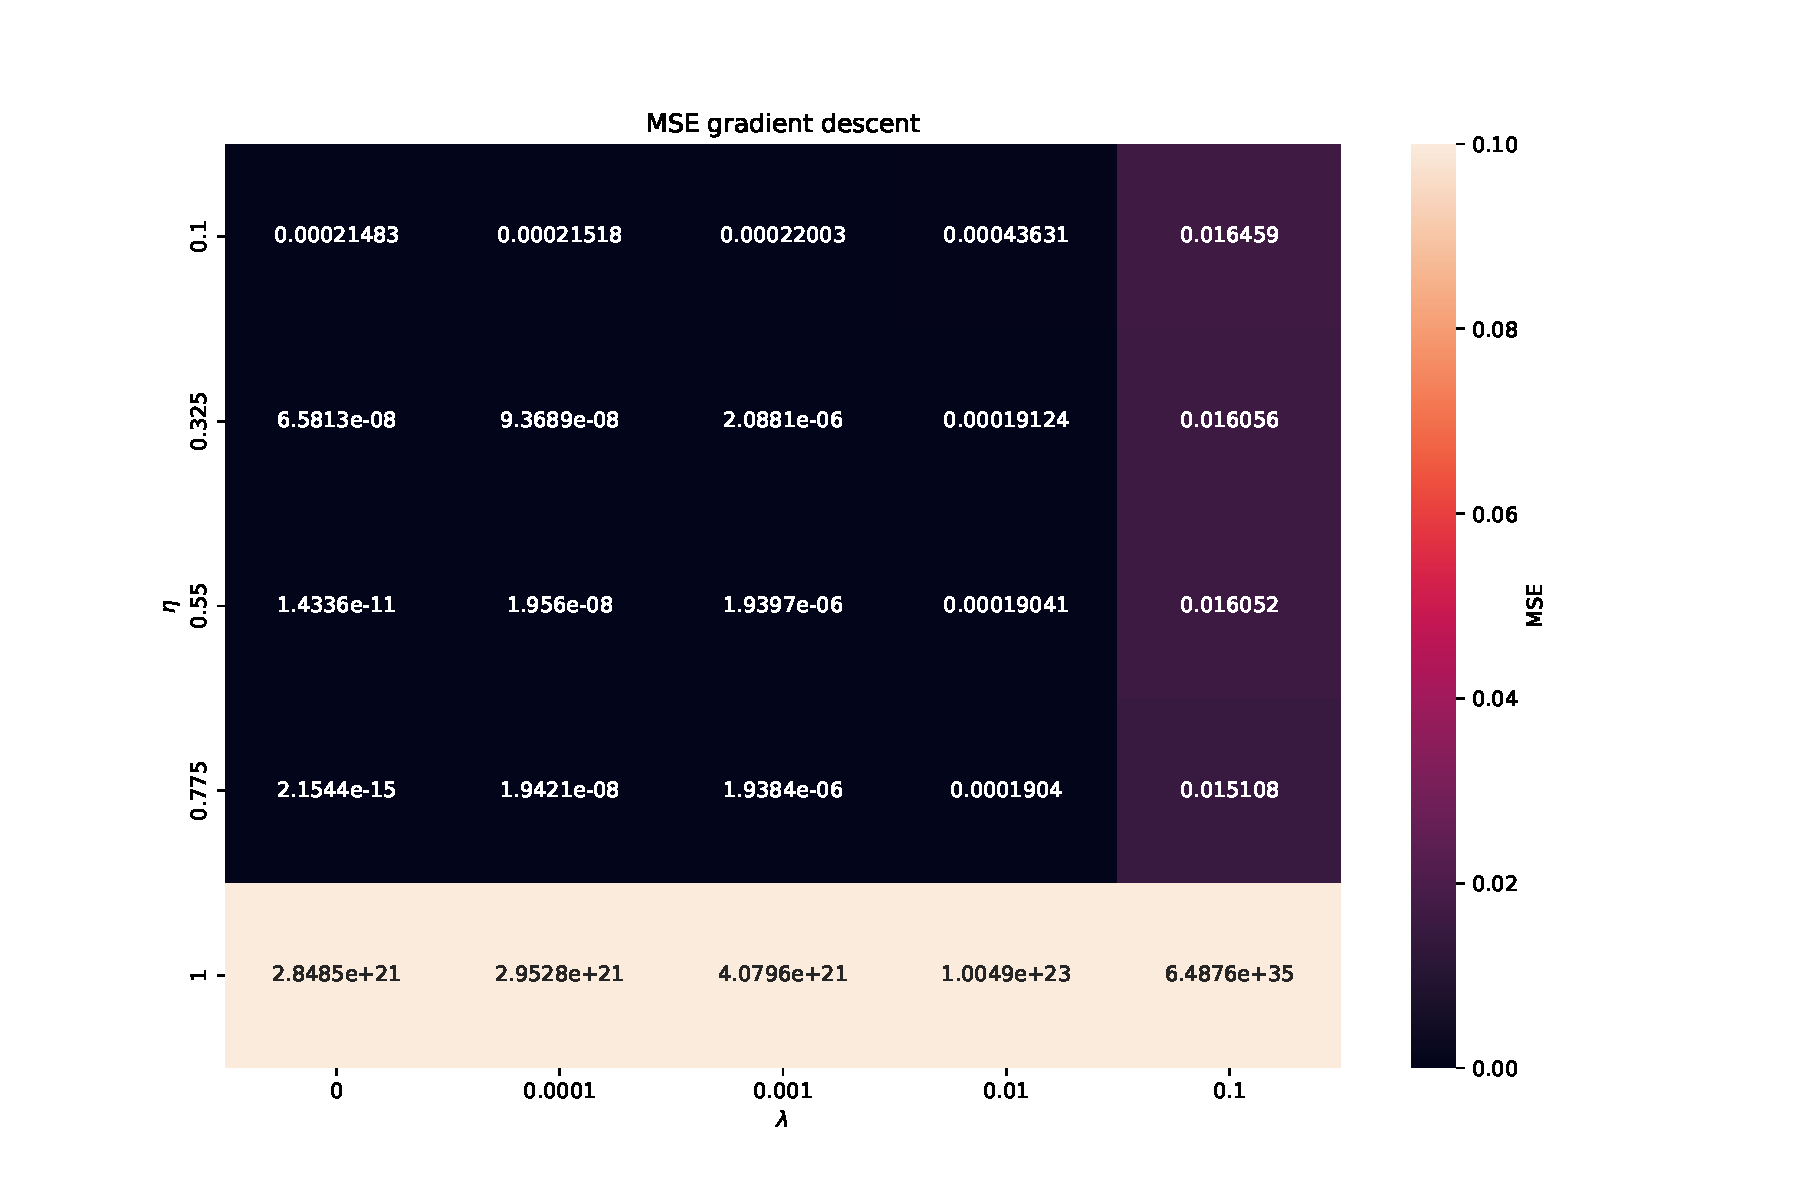
\includegraphics[width=0.8\textwidth]{Figures/PartA/gd_MSE(eta,lmb)}
\caption{Plain gradient descent MSE as a function of \(\eta \) and \(\lambda \).}
\label{fig:gd_MSE-eta-lmb-}
\end{figure}

\begin{figure}[H]
\centering
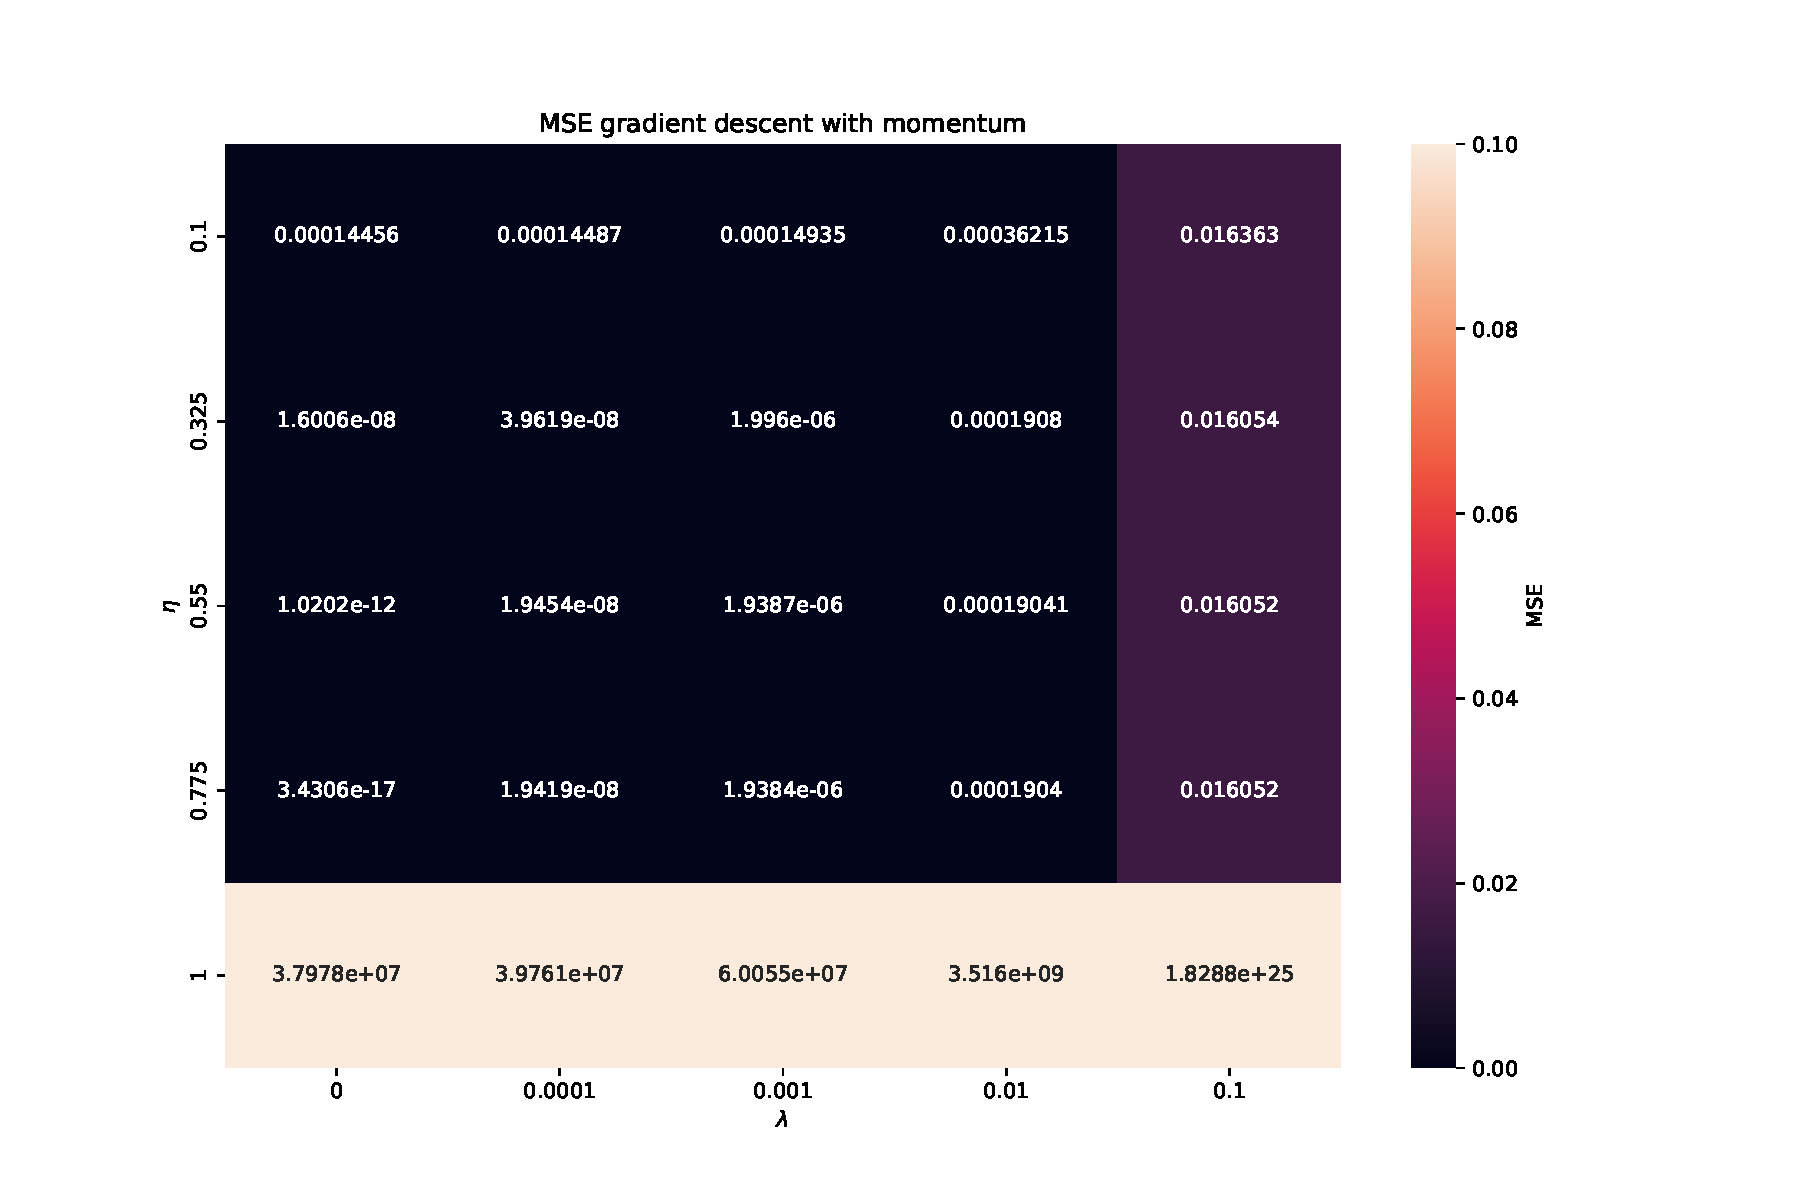
\includegraphics[width=0.8\textwidth]{Figures/PartA/gdm_MSE(eta,lmb)}
\caption{Gradient descent with momentum MSE as a function of \(\eta \) and \(\lambda \).}
\label{fig:gdm_MSE-eta-lmb-}
\end{figure}

\begin{figure}[H]
\centering
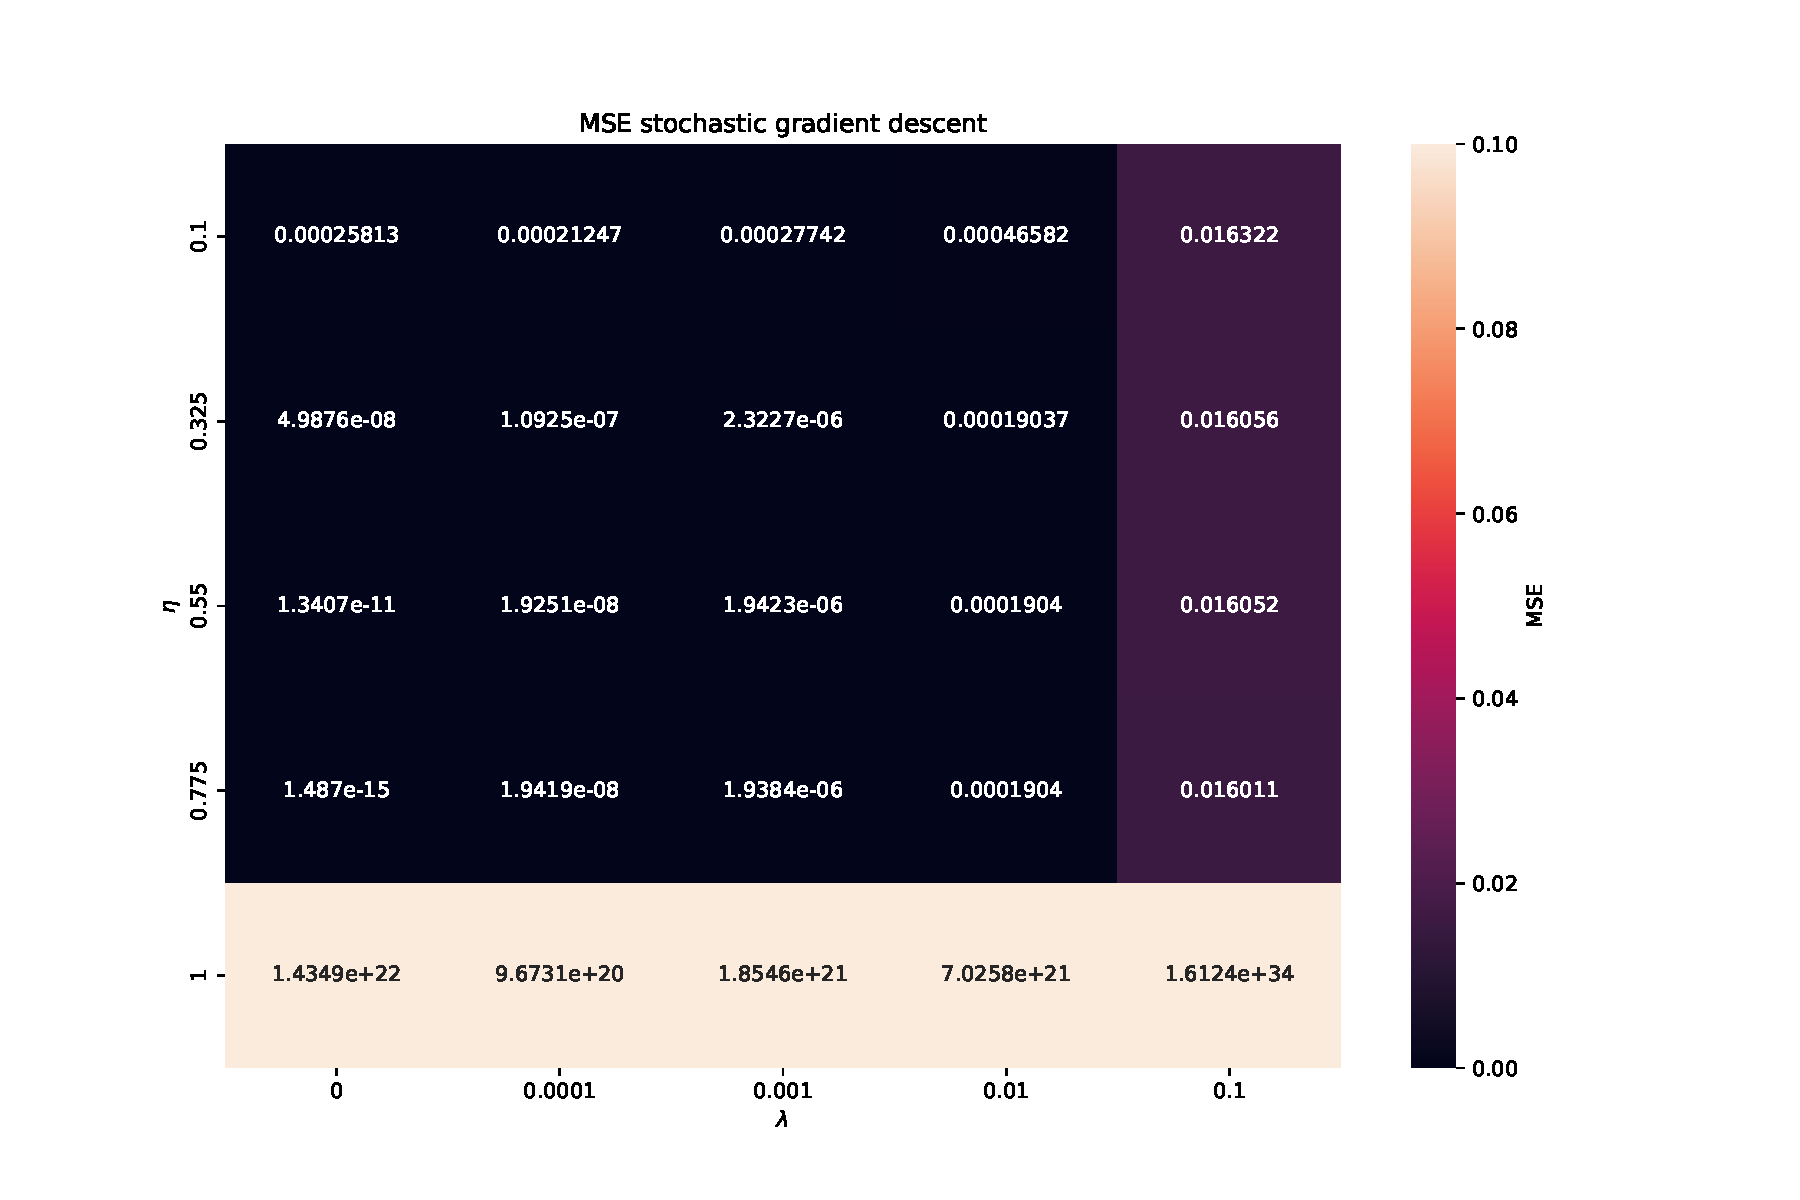
\includegraphics[width=0.8\textwidth]{Figures/PartA/sgd_MSE(eta,lmb)}
\caption{Plain stochastic gradient descent MSE as a function of \(\eta \) and \(\lambda \).}
\label{fig:sgd_MSE-eta-lmb-}
\end{figure}

\begin{figure}[H]
\centering
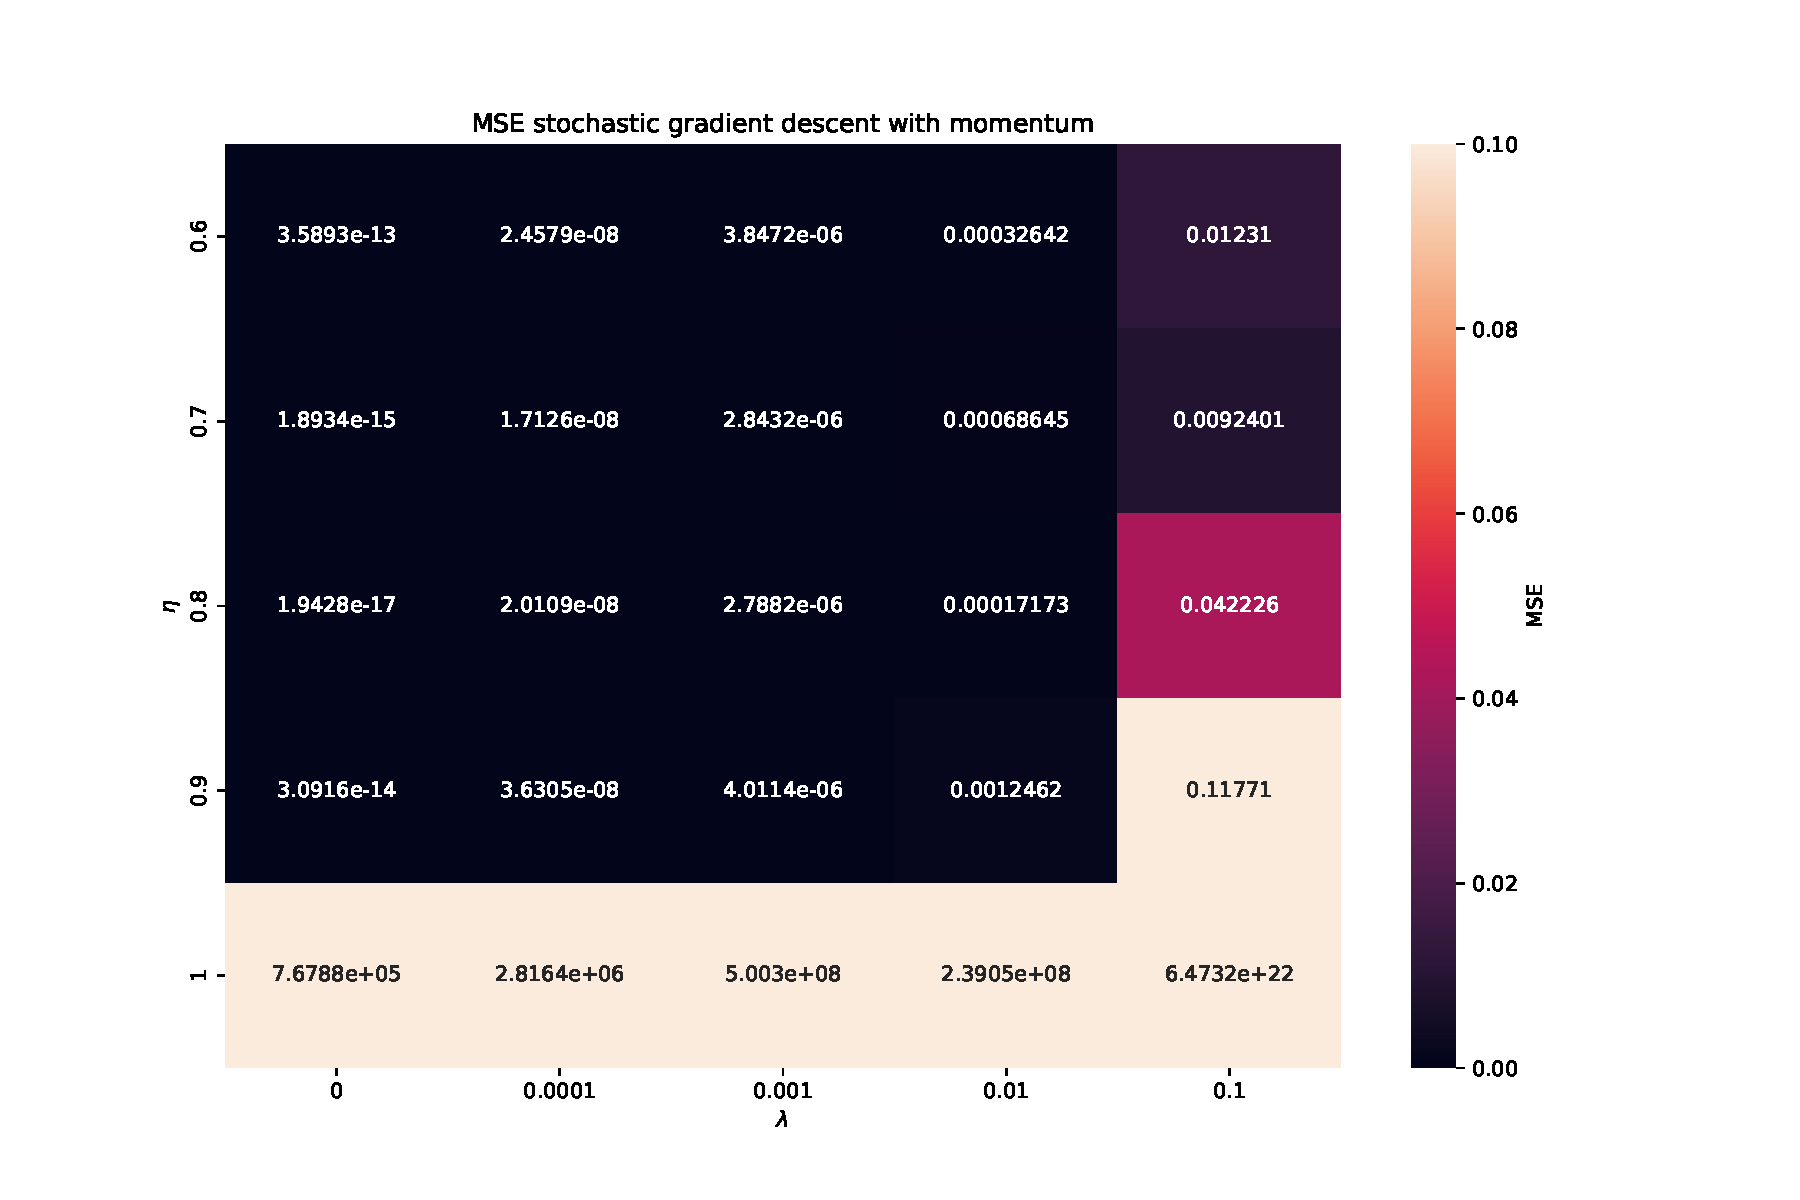
\includegraphics[width=0.8\textwidth]{Figures/PartA/sgdm_MSE(eta,lmb)}
\caption{Stochastic gradient descent with momentum MSE as a function of \(\eta \) and \(\lambda \).}
\label{fig:sgdm_MSE-eta-lmb-}
\end{figure}

Figure \ref{fig:gd_MSE-eta-lmb-}-\ref{fig:sgdm_MSE-eta-lmb-} shows MSE scores for 
stochastic gradient descent without ans with momentum, and stochastic gradient descent
without and with momentum, respectively. 
different learning rates \(\eta \) and L2-regularzation parameters \(\lambda \). 


\begin{figure}[H]
\centering
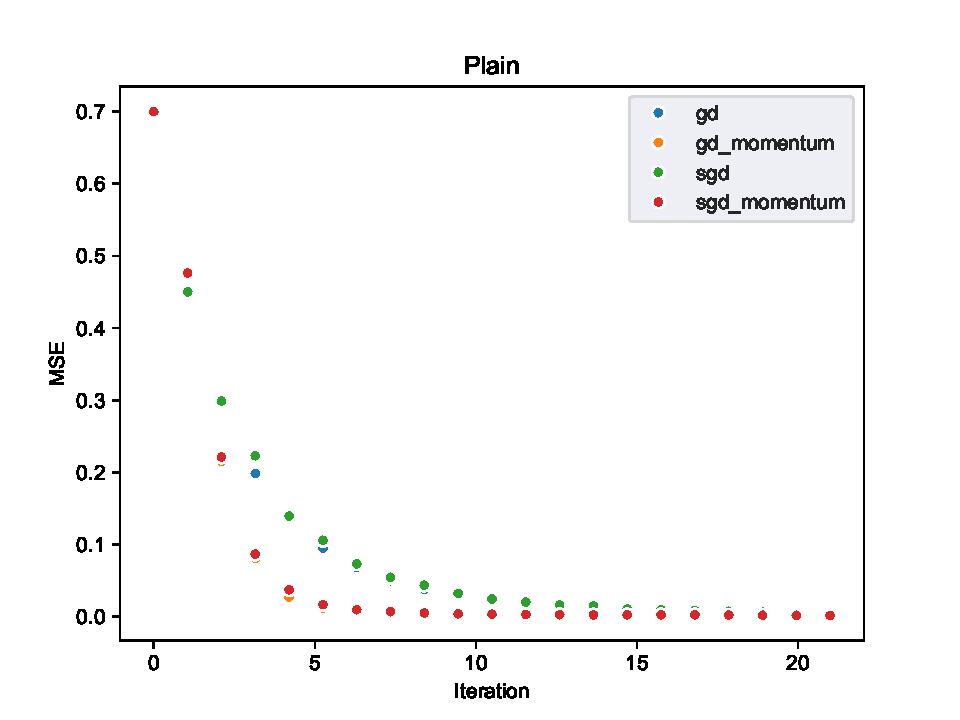
\includegraphics[width=0.8\textwidth]{Figures/PartA/PlainMSE(iter).pdf}
\caption{MSE as a function of iterations for plain and stochastic gradient descent with and without momentum}
\label{fig:PlainMSE-iter-pdf}
\end{figure}

\begin{figure}[H]
\centering
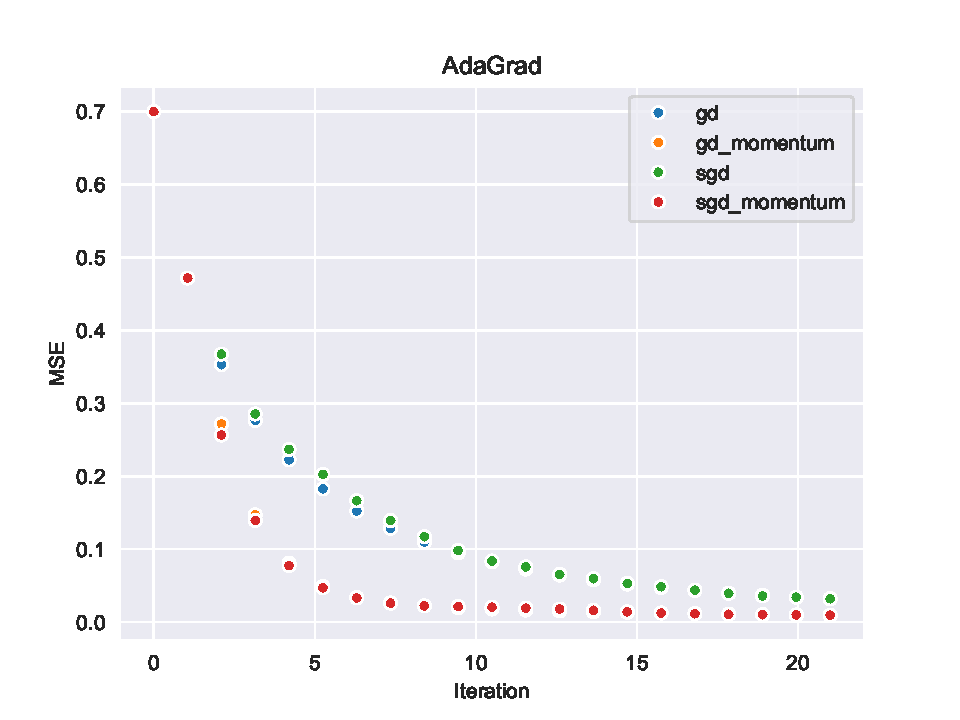
\includegraphics[width=0.8\textwidth]{Figures/PartA/AdaGradMSE(iter).pdf}
\caption{MSE as a function of iterations using tuning method AdaGrad for plain and stochastic gradient descent with and without momentum}
\label{fig:AdaGradMSE-iter-pdf}
\end{figure}

\begin{figure}[H]
\centering
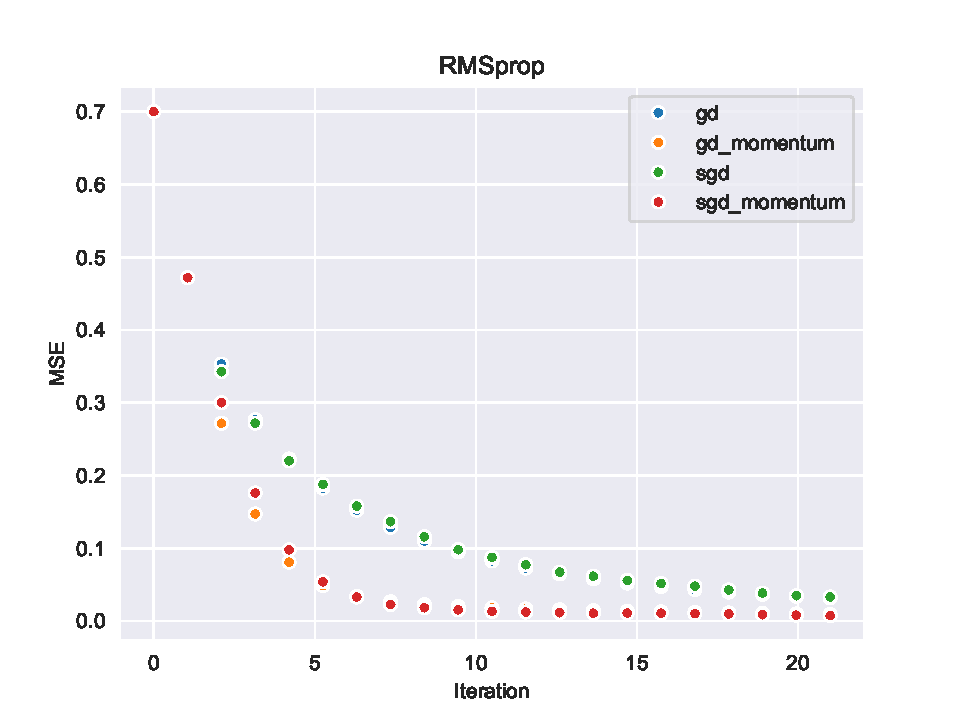
\includegraphics[width=0.8\textwidth]{Figures/PartA/RMSpropMSE(iter).pdf}
\caption{MSE as a function of iterations using tuning method RMSprop for plain and stochastic gradient descent with and without momentum}
\label{fig:RMSpropMSE-iter-pdf}
\end{figure}

\begin{figure}[H]
\centering
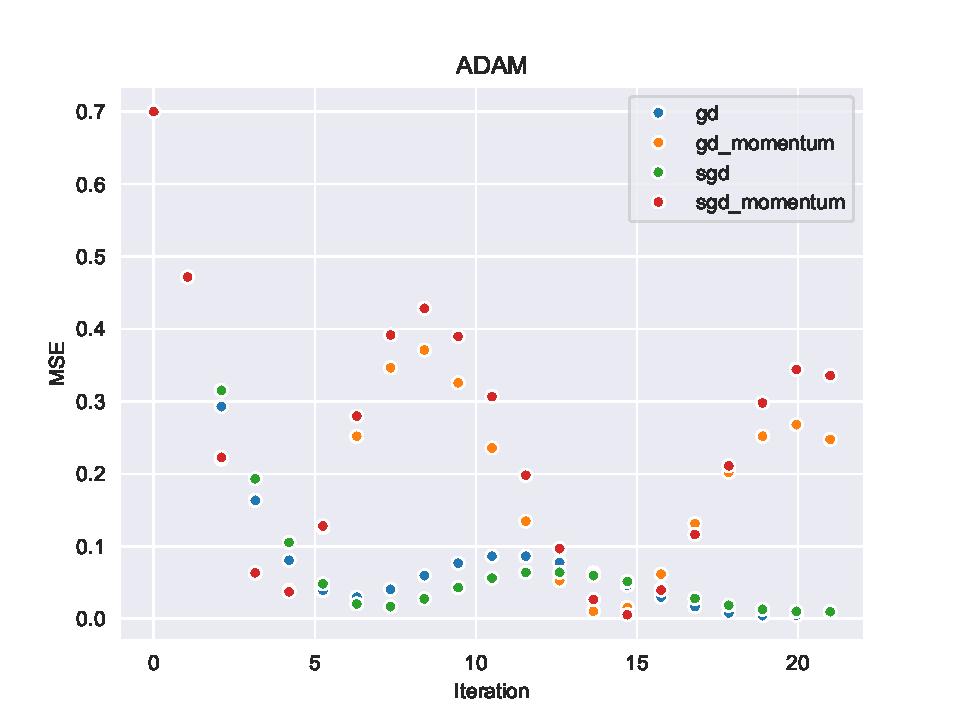
\includegraphics[width=0.8\textwidth]{Figures/PartA/ADAMMSE(iter).pdf}
\caption{MSE as a function of iterations using tuning method ADAM for plain and stochastic gradient descent with and without momentum}
\label{fig:ADAMMSE-iter-pdf}
\end{figure}



\begin{figure}[H]
\centering
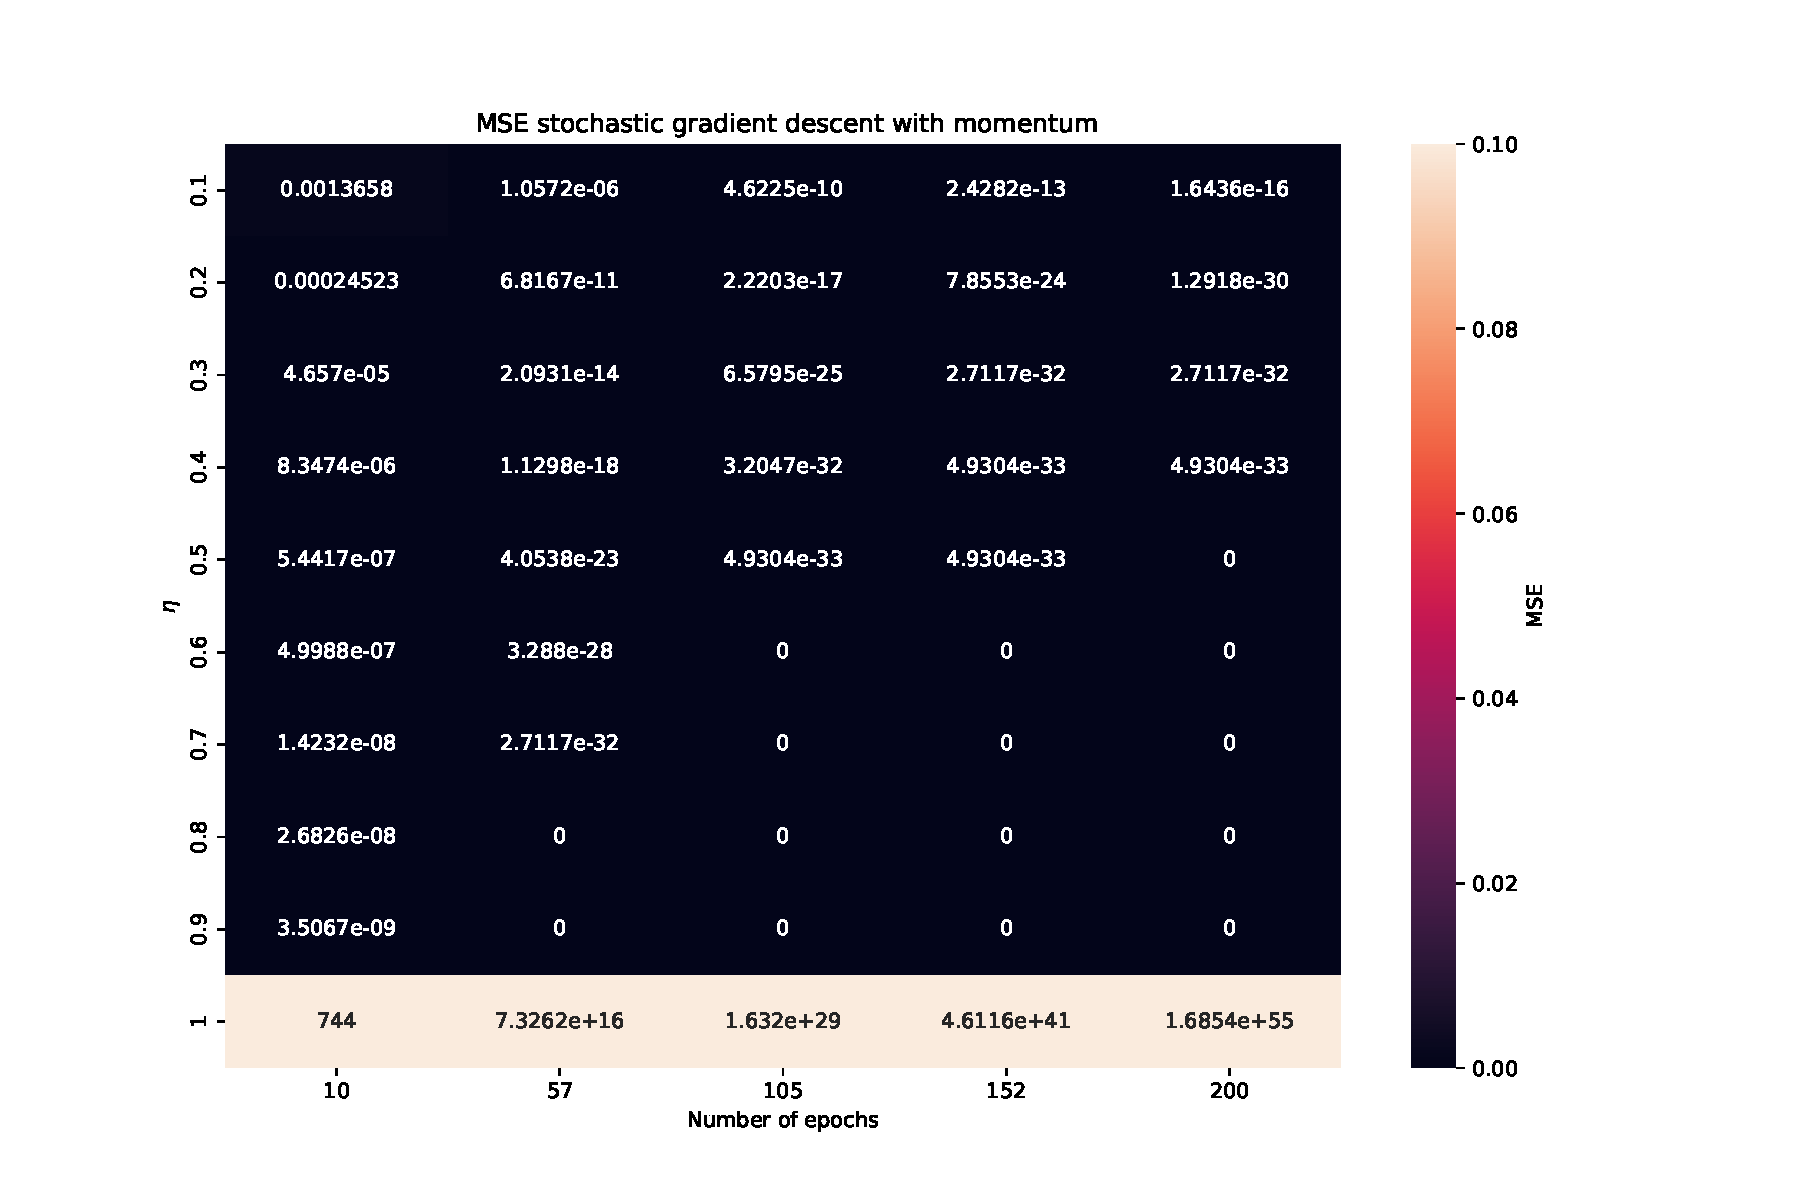
\includegraphics[width=0.8\textwidth]{Figures/PartA/_sgdm_MSE(eta,epochs)}
\caption{Stochastic gradient descent with momentum MSE as a function of epoch number and \(\eta \)	 }
\label{fig:_sgdm_MSE-eta-epochs-}
\end{figure}

\begin{figure}[H]
\centering
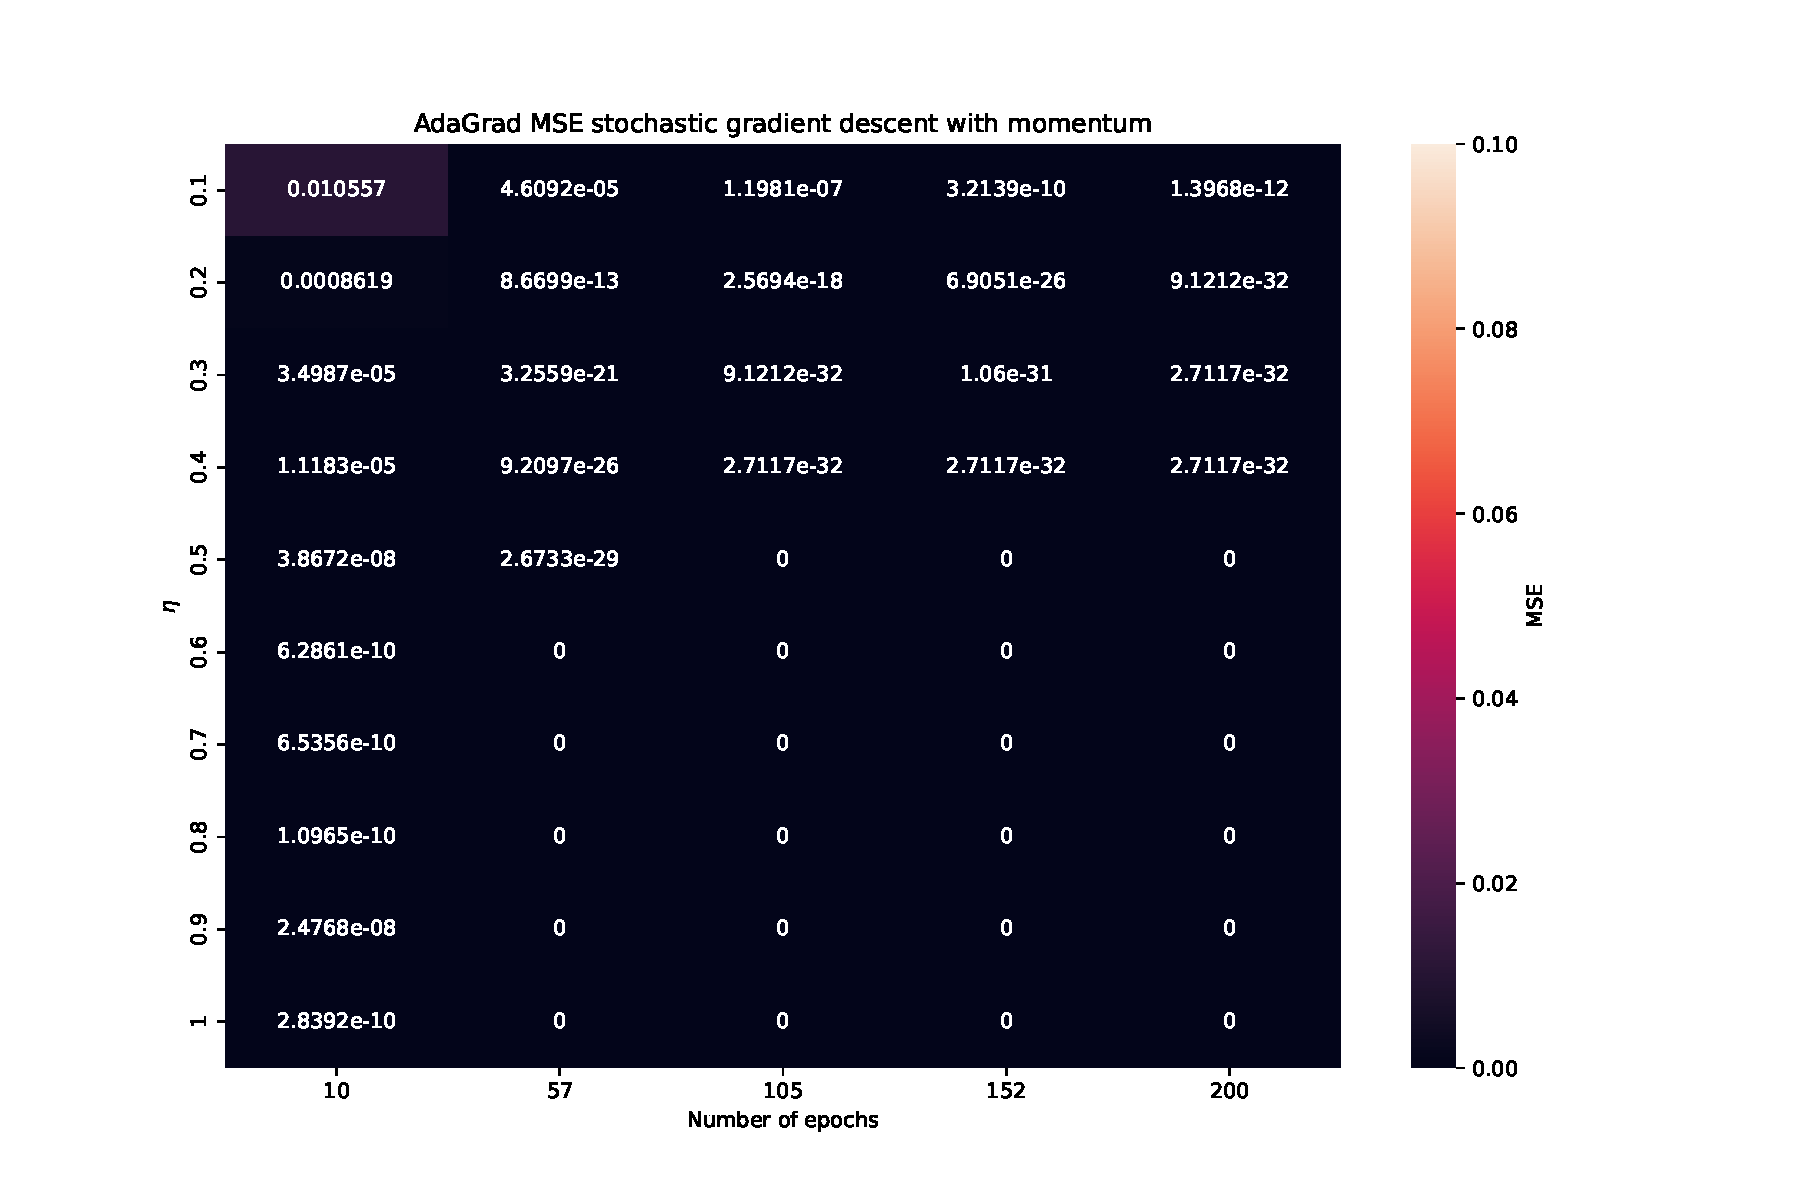
\includegraphics[width=0.8\textwidth]{Figures/PartA/AdaGrad_sgdm_MSE(eta,epochs)}
\caption{Stochastic gradient descent, with momentum and tuning method AdaGrad, MSE as a function of epoch number and \(\eta \)	 }
\label{fig:AdaGrad_sgdm_MSE-eta-epochs-}
\end{figure}

\begin{figure}[H]
\centering
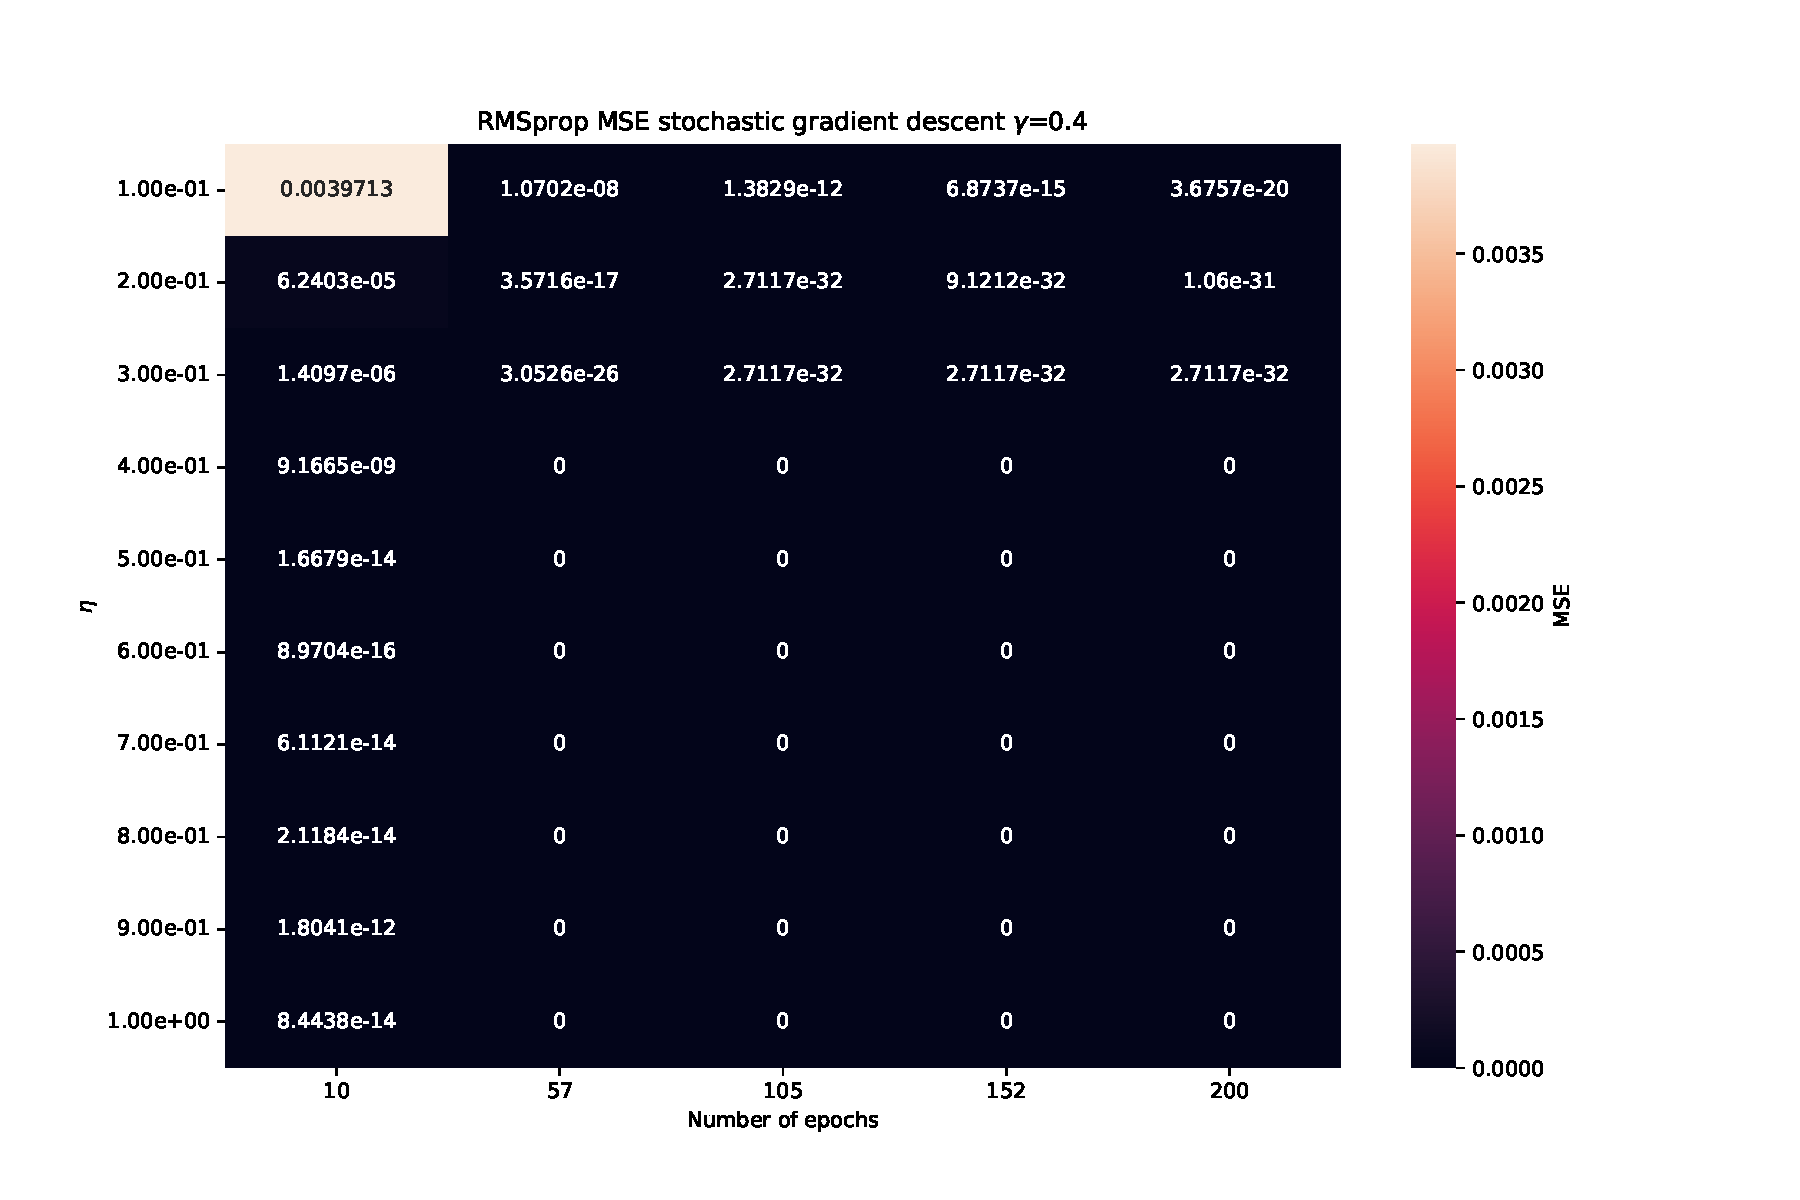
\includegraphics[width=0.8\textwidth]{Figures/PartA/RMSprop_sgdm_MSE(eta,epochs)}
\caption{Stochastic gradient descent, with momentum and tuning method RMS\_prop, MSE as a function of epoch number and \(\eta \)	 }
\label{fig:RMSprop_sgdm_MSE-eta-epochs-}
\end{figure}

\begin{figure}[H]
\centering
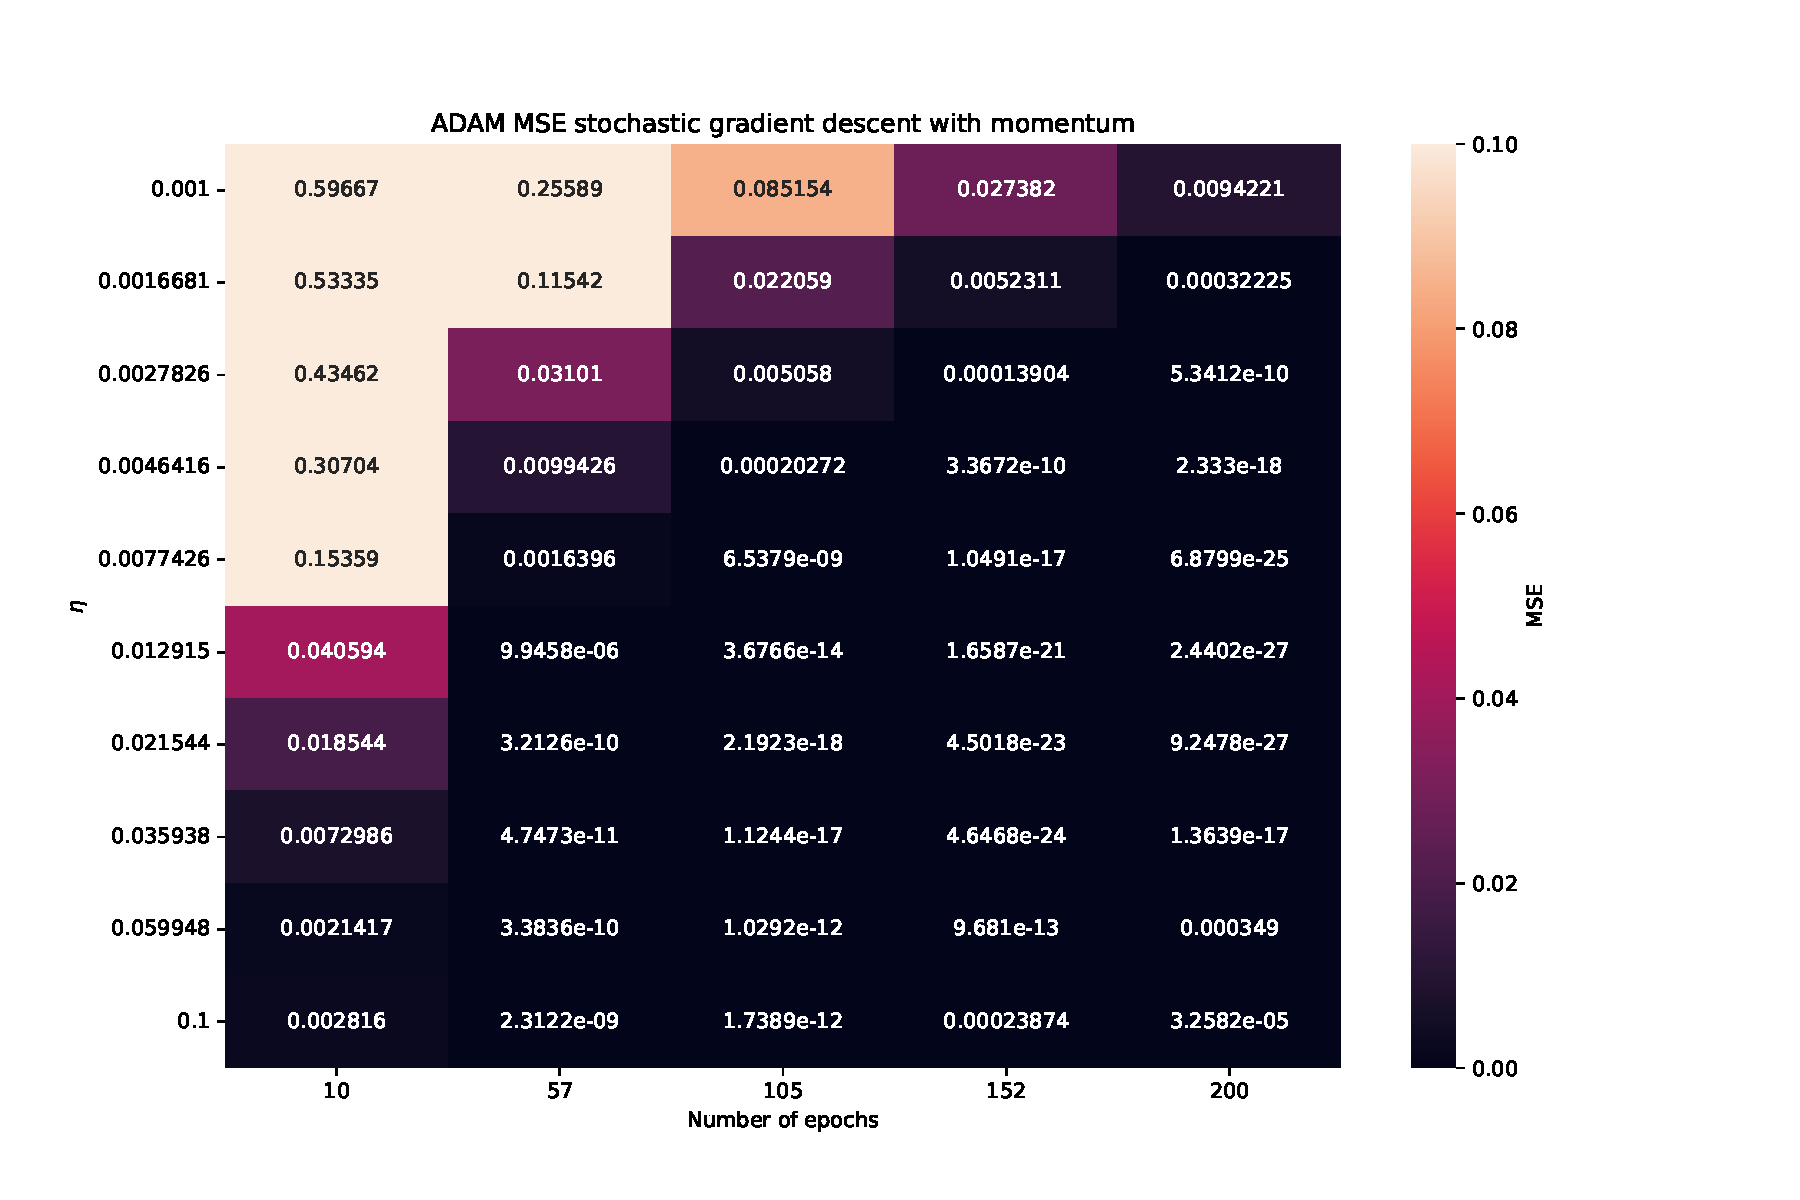
\includegraphics[width=0.8\textwidth]{Figures/PartA/ADAM_sgdm_MSE(eta,epochs)}
\caption{Stochastic gradient descent, with momentum and tuning method ADAM, MSE as a function of epoch number and \(\eta \)	 }
\label{fig:ADAM_sgdm_MSE-eta-epochs-}
\end{figure}


\subsection{Neural Network Regression}

\begin{figure}[htpb]
\begin{subfigure}{.5\textwidth}
  \centering
  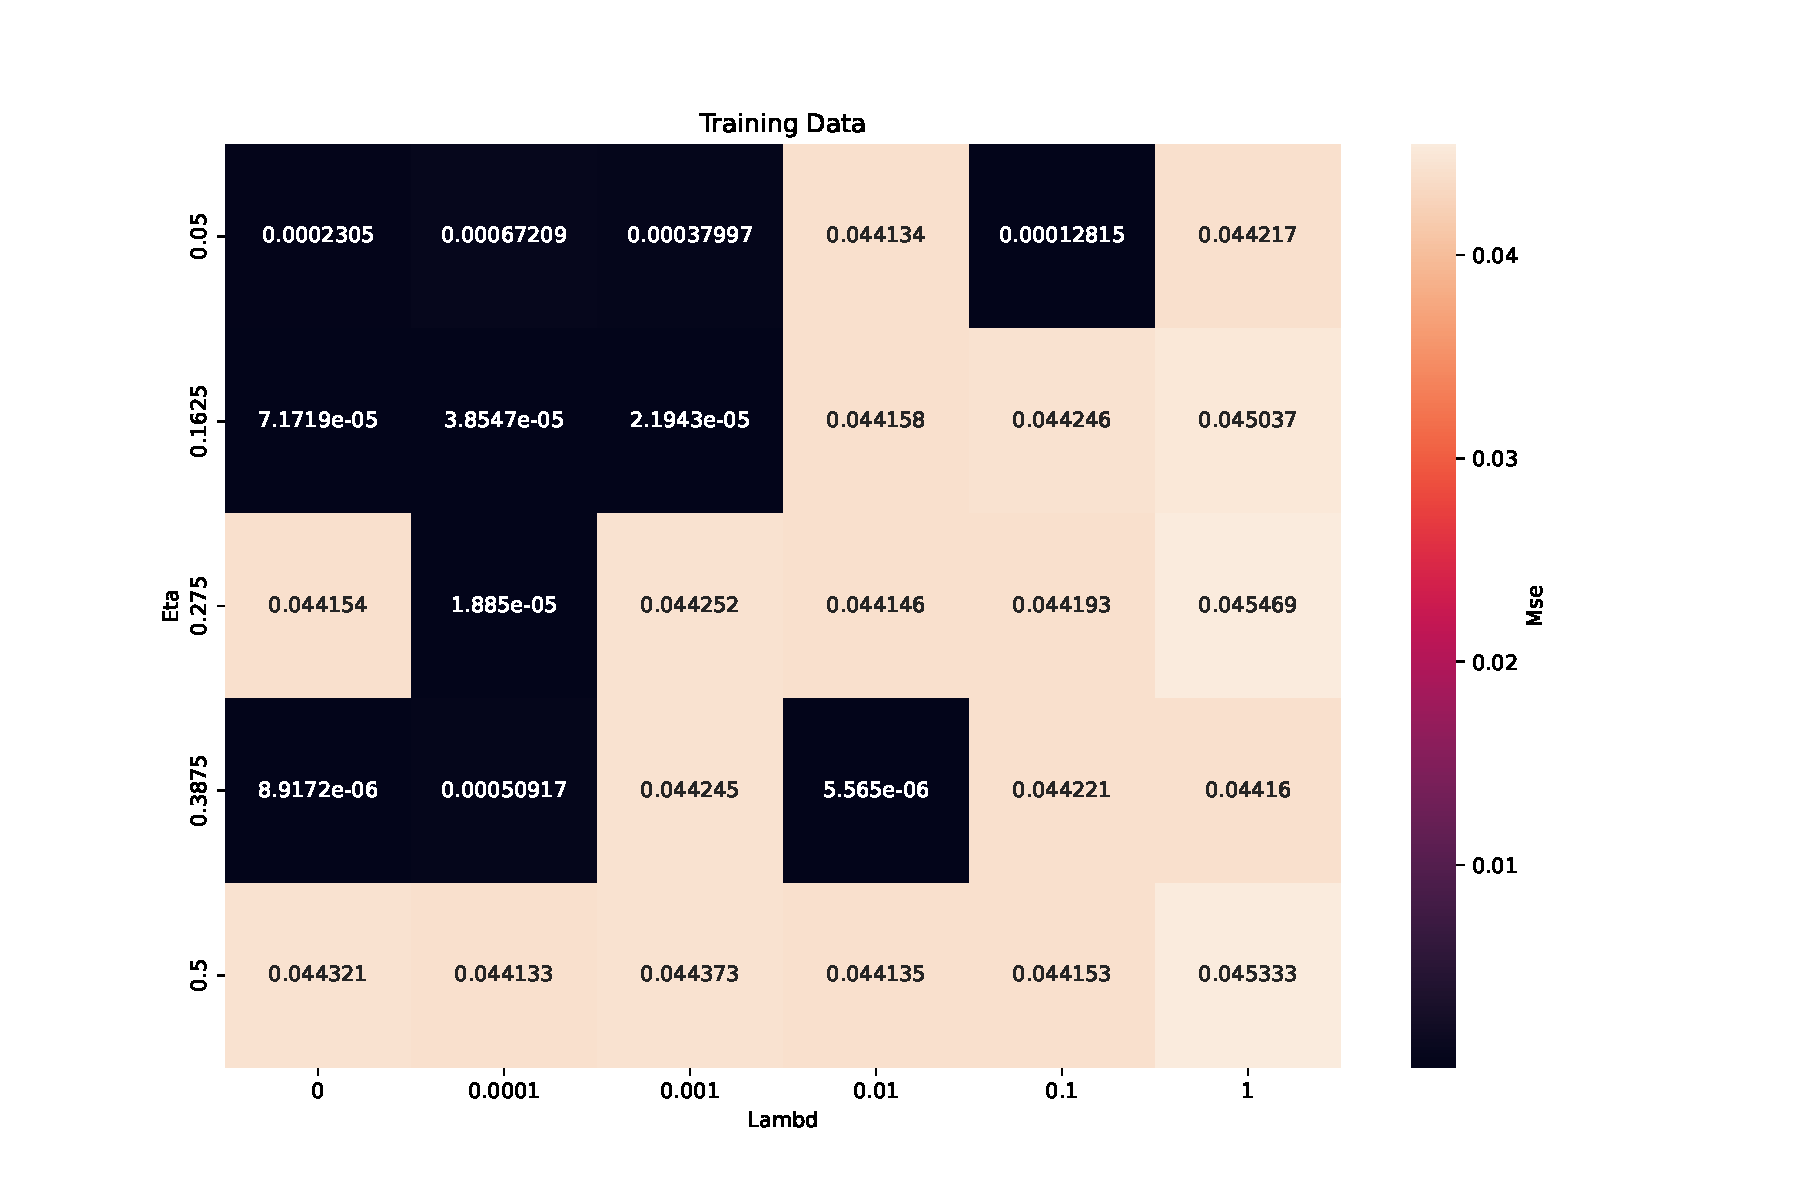
\includegraphics[width=1.2\linewidth]{Figures/PartB/train_sigmoid_MSE(eta,lmb)}
  \caption{Train MSE}
  \label{fig:train_sigmoid_MSE-eta-lmb-}
\end{subfigure}%
\begin{subfigure}{.5\textwidth}
  \centering
  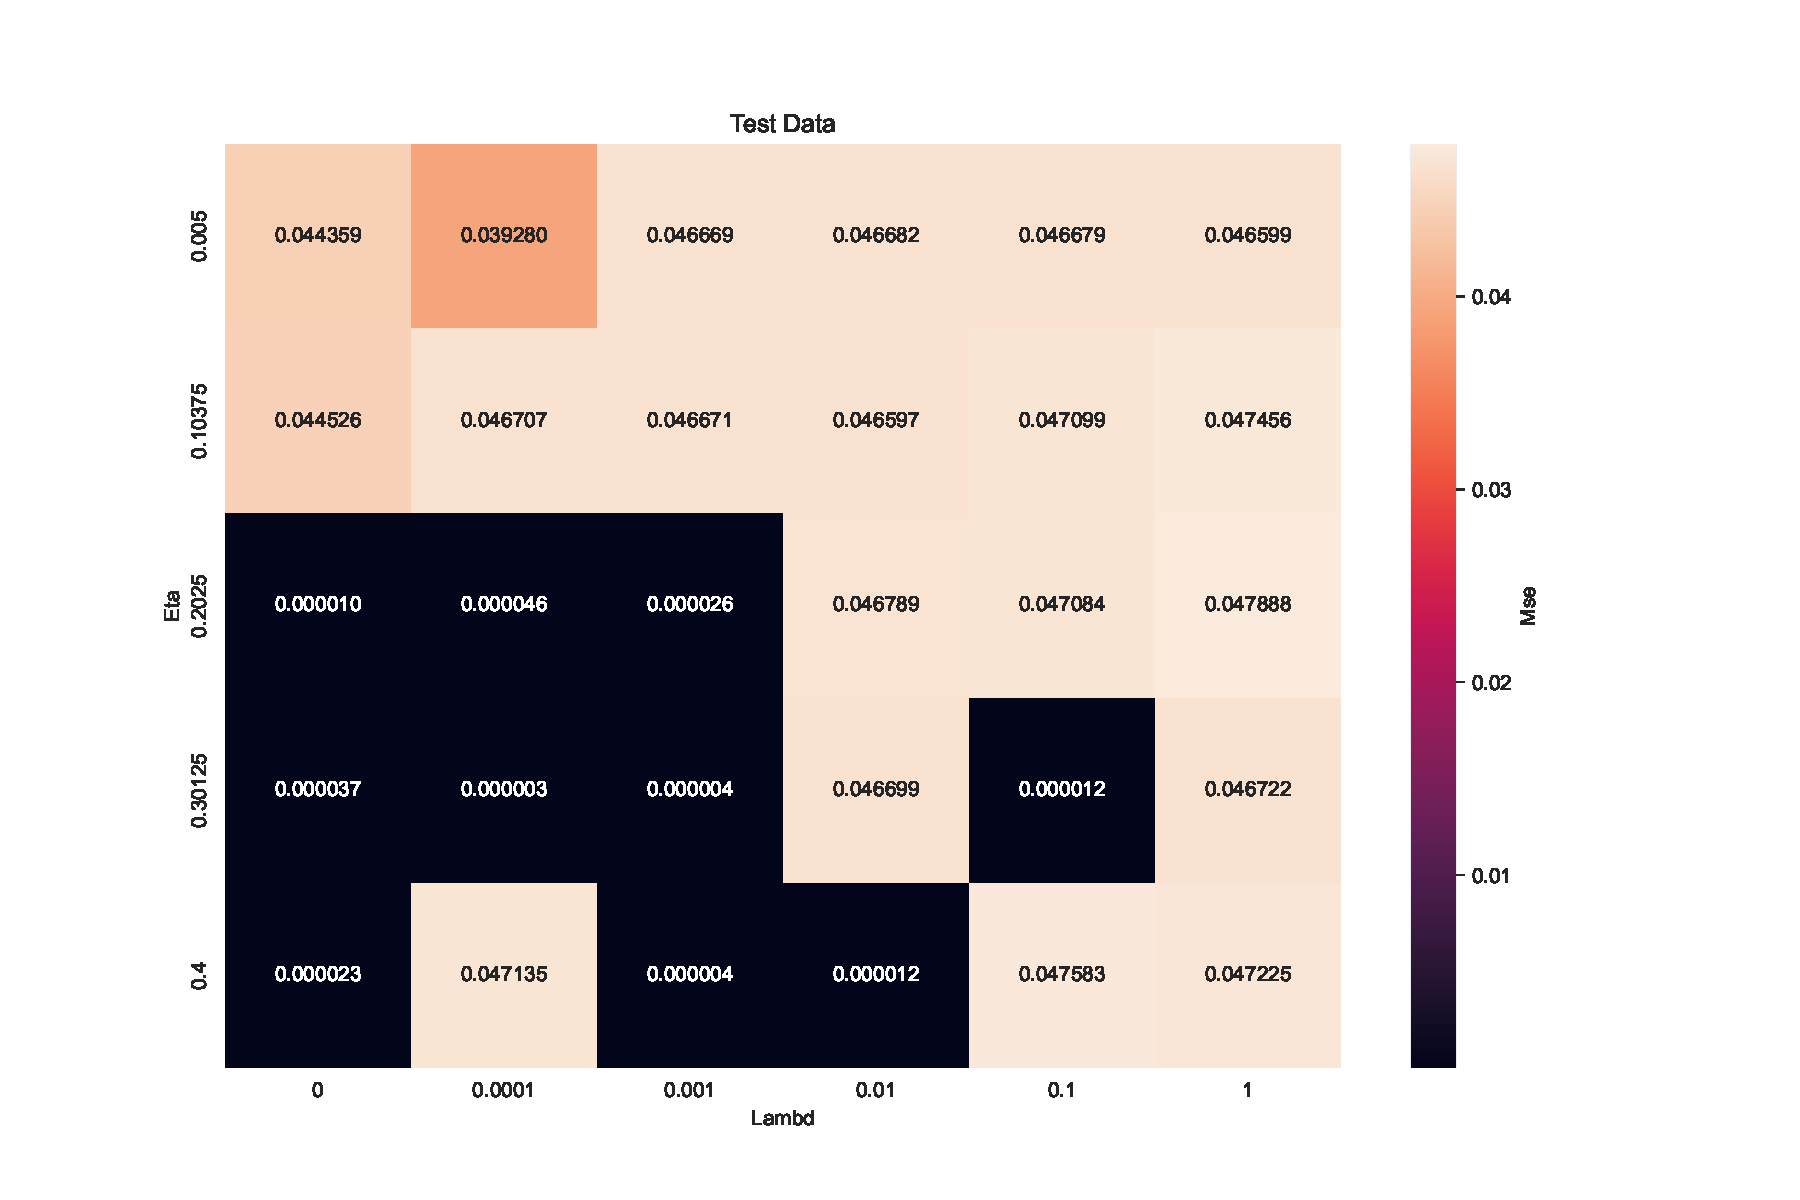
\includegraphics[width=1.2\linewidth]{Figures/PartB/test_sigmoid_MSE(eta,lmb)}
  \caption{Test MSE}
  \label{fig:test_sigmoid_MSE-eta-lmb-}
\end{subfigure}
\caption{Neural network with activation function Sigmoid MSE as a function of \(\eta \) and \(\lambda \) }
\label{fig:Sigmoid_MSE}
\end{figure}

\begin{figure}[htpb]
\begin{subfigure}{.5\textwidth}
  \centering
  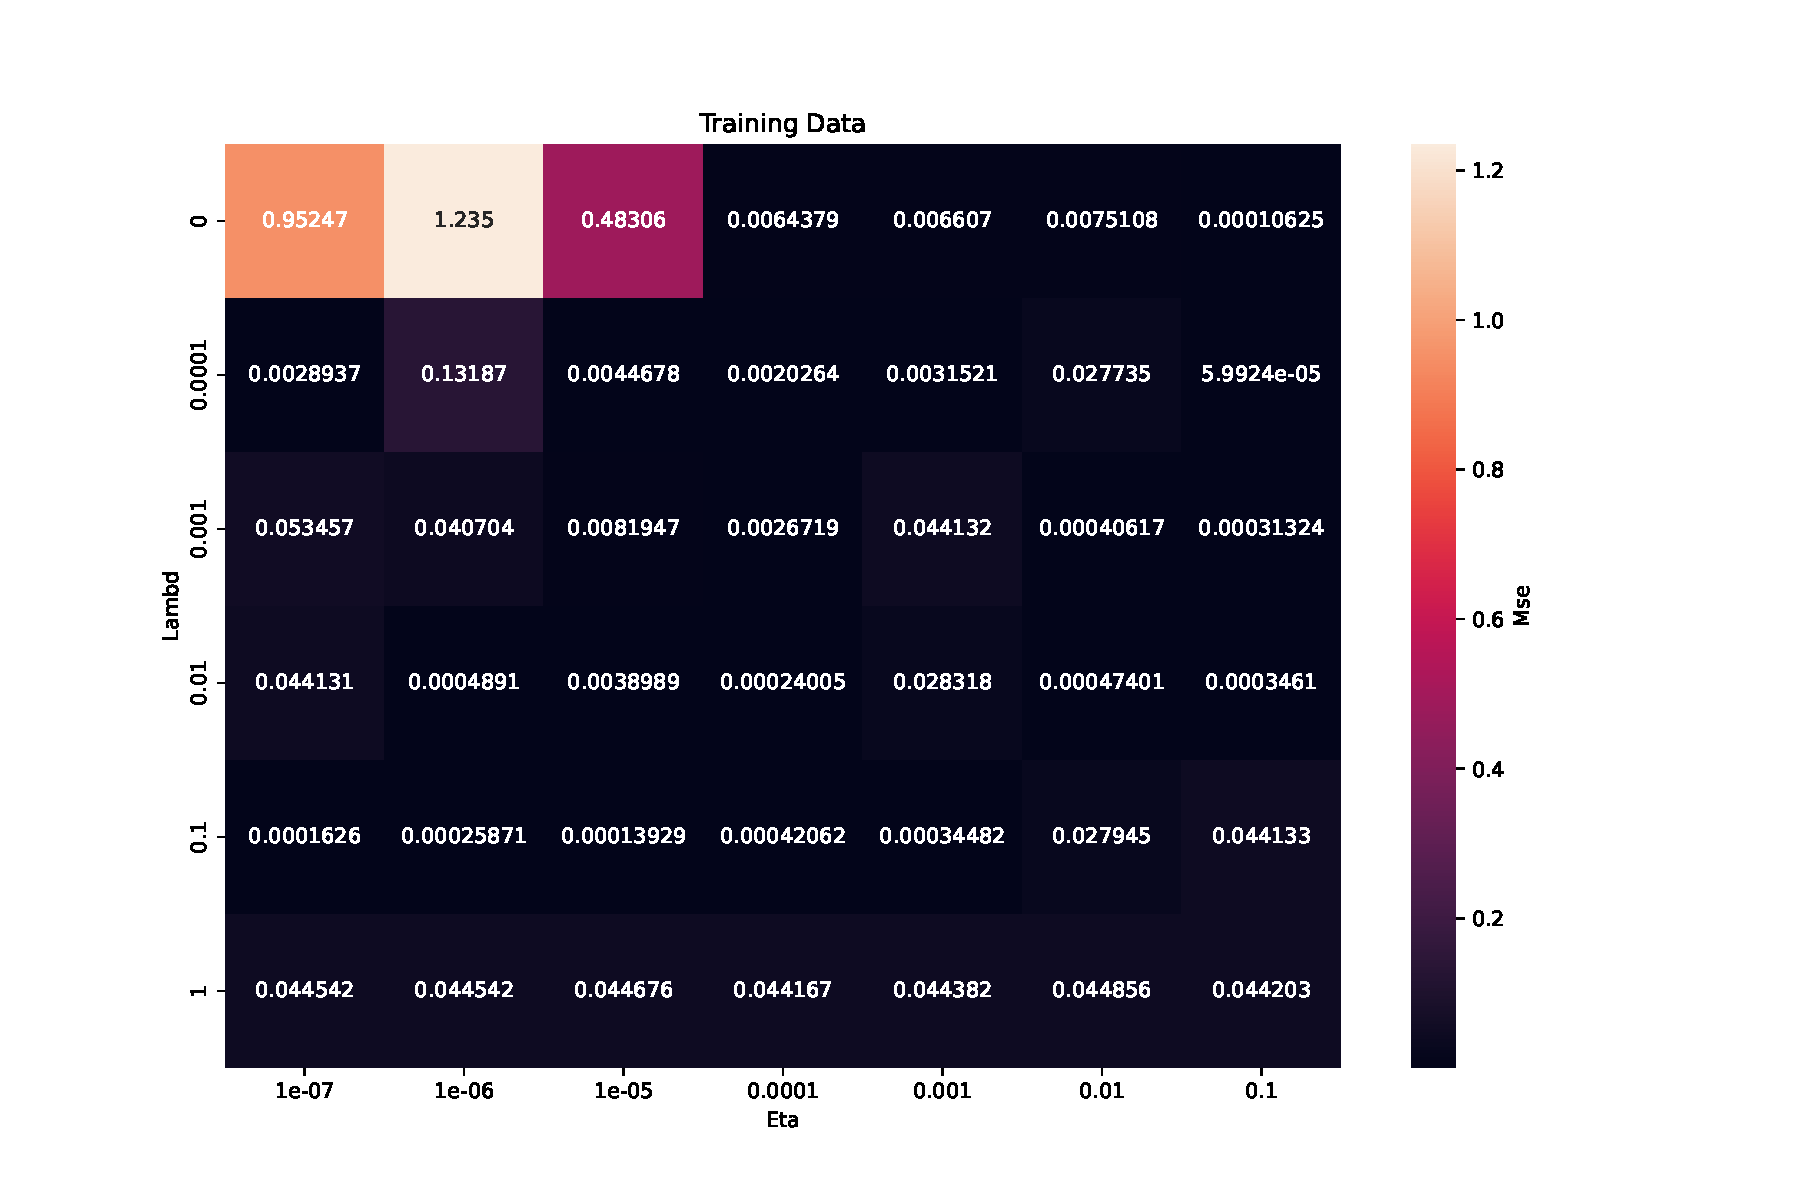
\includegraphics[width=1.2\linewidth]{Figures/PartB/train_relu_MSE(eta,lmb)}
  \caption{Train MSE}
  \label{fig:train_relu_MSE-eta-lmb-}
\end{subfigure}%
\begin{subfigure}{.5\textwidth}
  \centering
  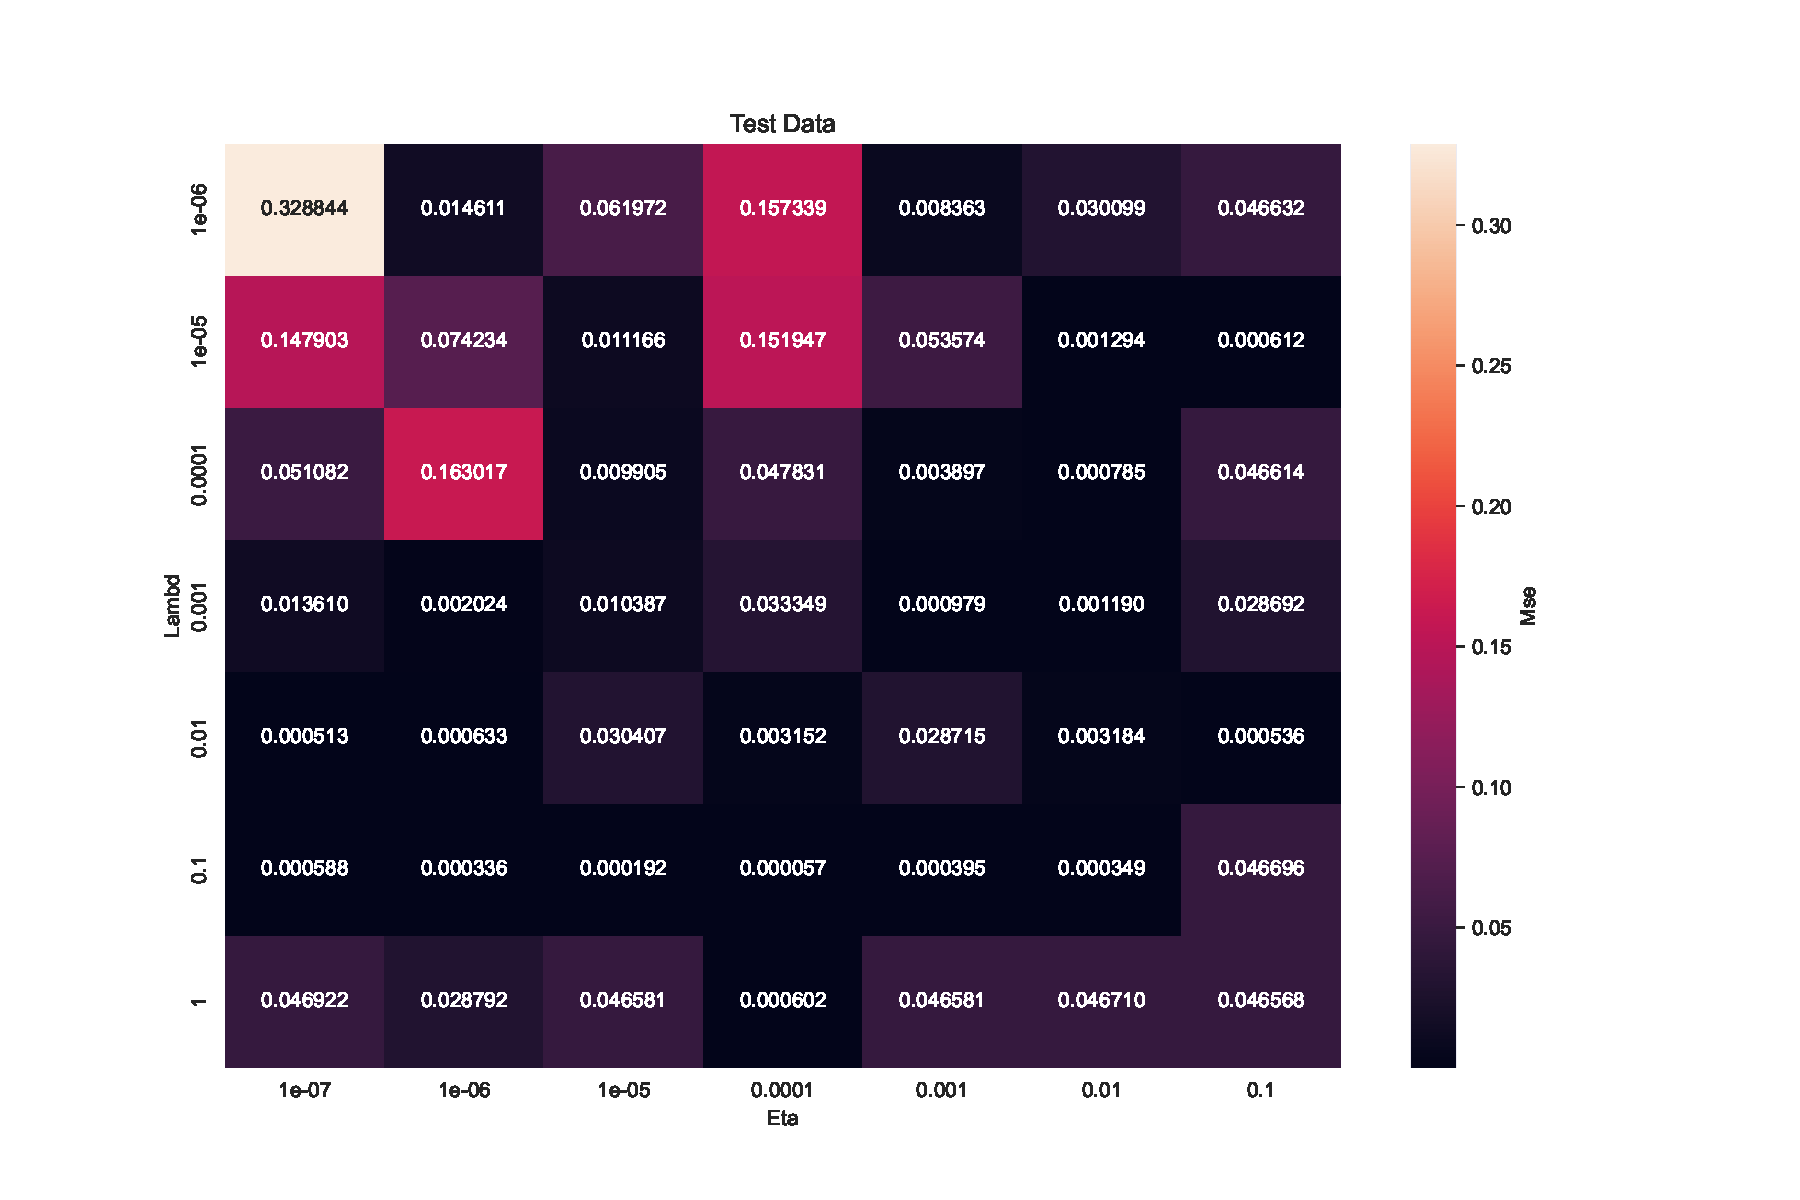
\includegraphics[width=1.2\linewidth]{Figures/PartB/test_relu_MSE(eta,lmb)}
  \caption{Test MSE}
  \label{fig:test_relu_MSE-eta-lmb-}
\end{subfigure}
\caption{Neural network with activation function relu MSE as a function of \(\eta \) and \(\lambda \) }
\label{fig:relu_MSE}
\end{figure}

\begin{figure}[htpb]
\begin{subfigure}{.5\textwidth}
  \centering
  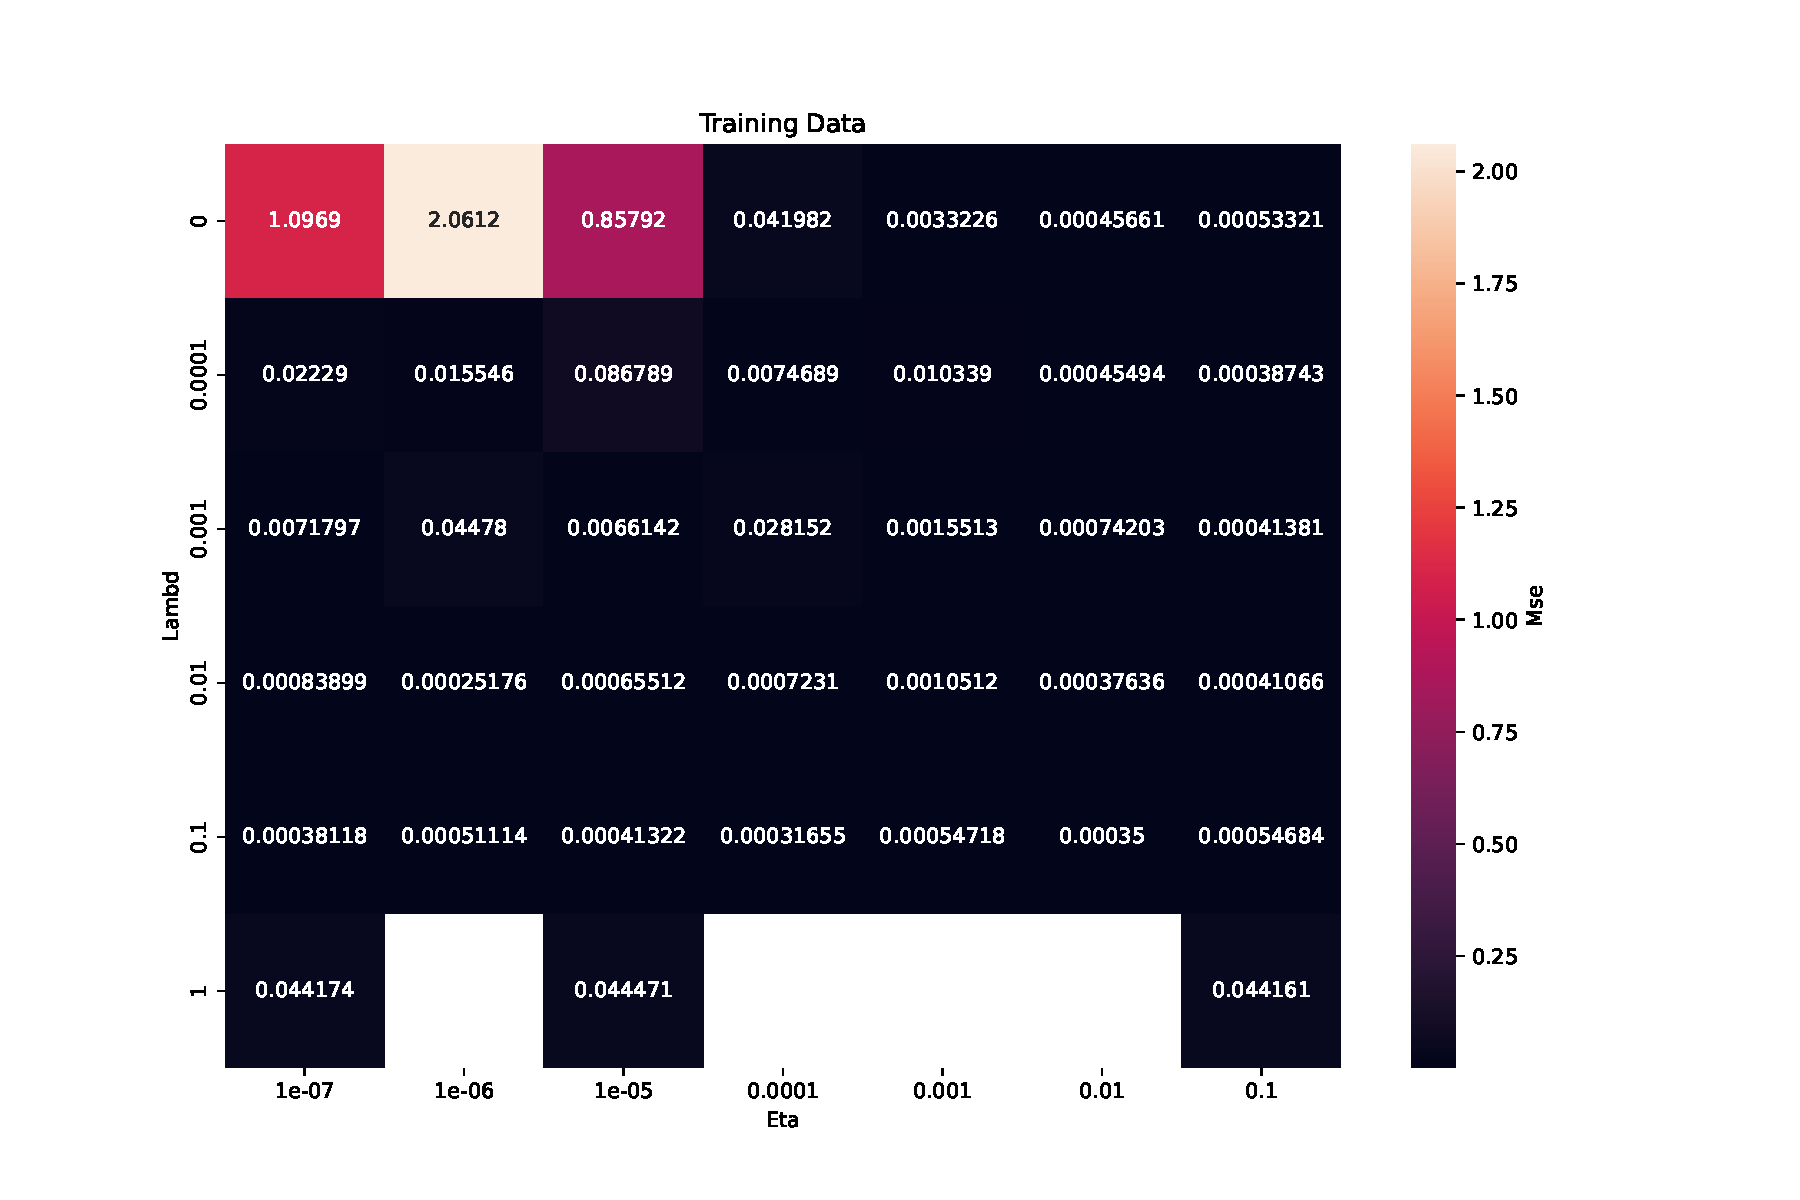
\includegraphics[width=1.2\linewidth]{Figures/PartB/train_leaky_relu_MSE(eta,lmb)}
  \caption{Train MSE}
  \label{fig:train_leaky_relu_MSE-eta-lmb-}
\end{subfigure}%
\begin{subfigure}{.5\textwidth}
  \centering
  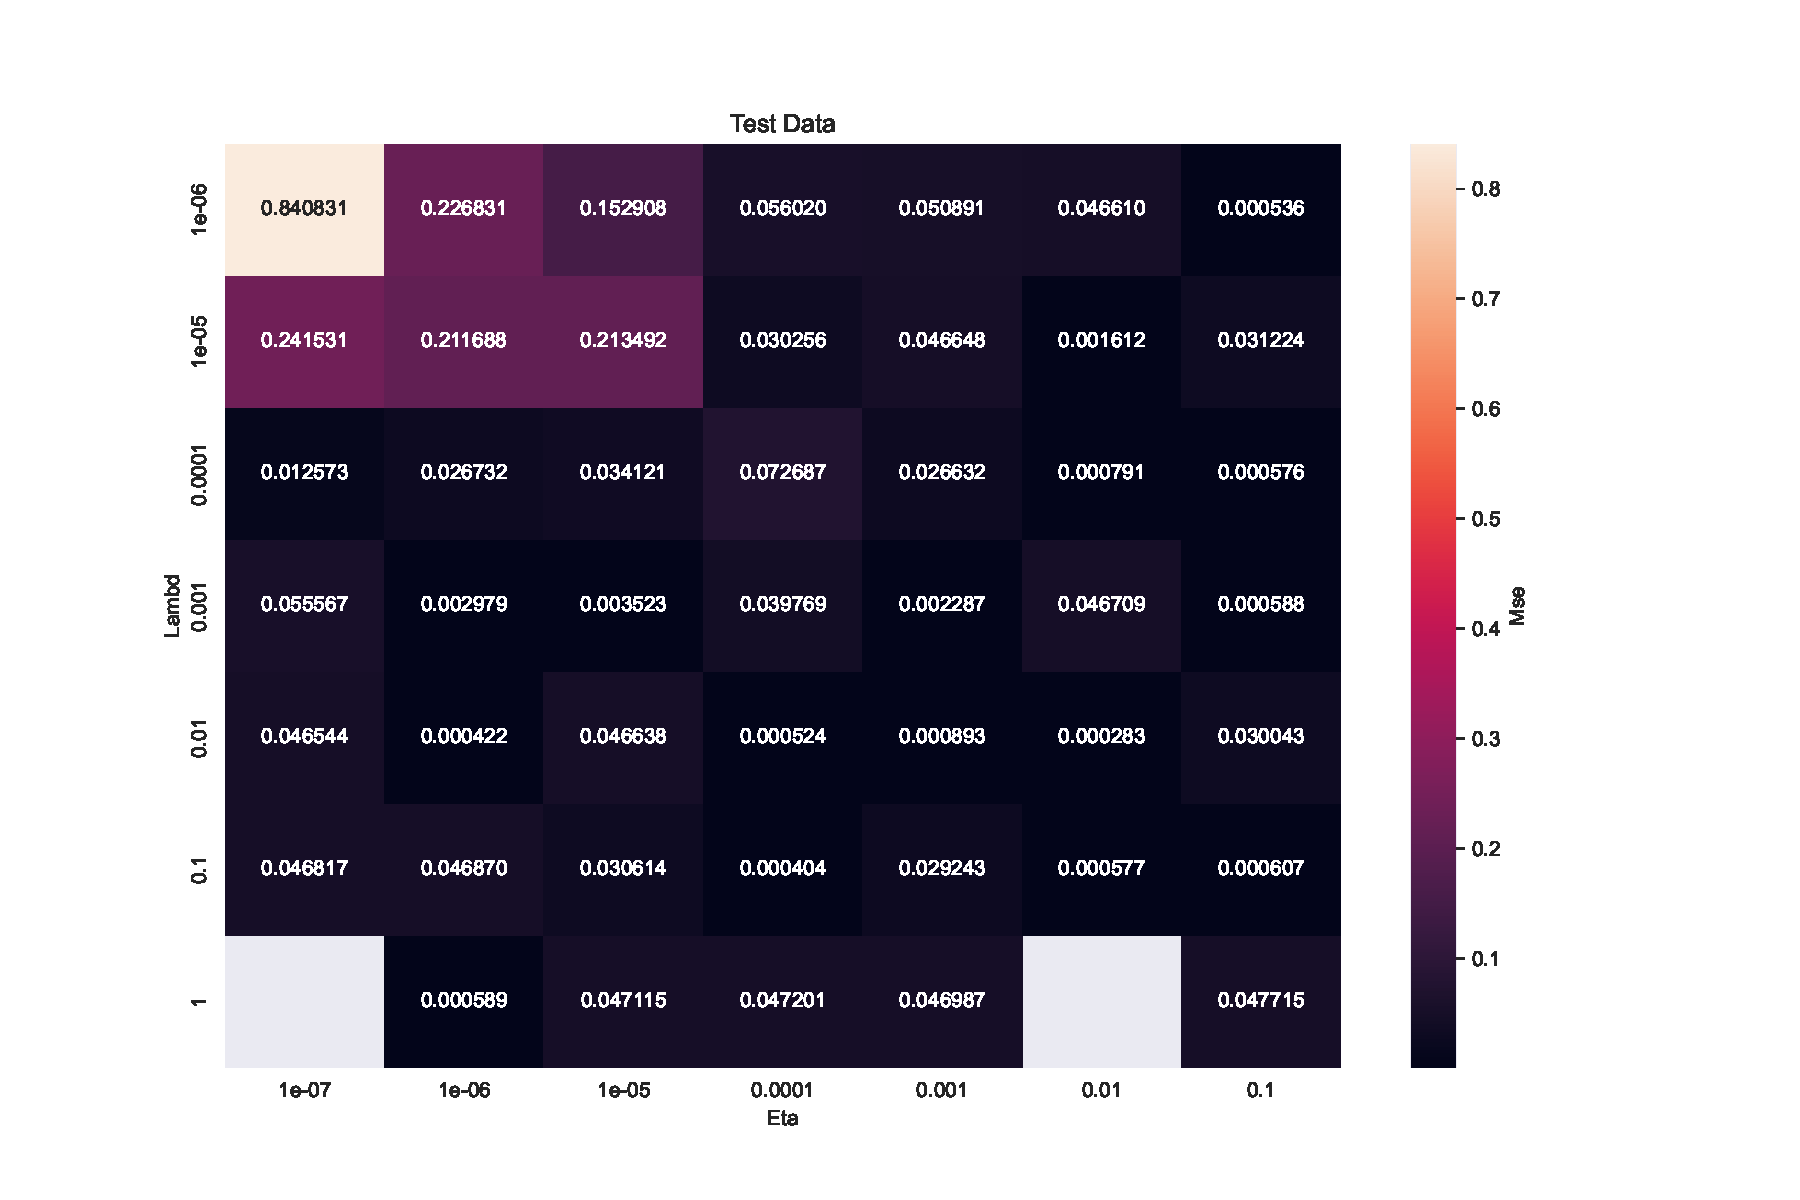
\includegraphics[width=1.2\linewidth]{Figures/PartB/test_leaky_relu_MSE(eta,lmb)}
  \caption{Test MSE}
  \label{fig:test_leaky_relu_MSE-eta-lmb-}
\end{subfigure}
\caption{Neural network with activation function leaky relu MSE as a function of \(\eta \) and \(\lambda \) }
\label{fig:leaky_relu_MSE}
\end{figure}






\subsection{Classification}


%  ____            _         _ 
% |  _ \ __ _ _ __| |_    __| |
% | |_) / _` | '__| __|  / _` |
% |  __/ (_| | |  | |_  | (_| |
% |_|   \__,_|_|   \__|  \__,_|
%                              

%%%%%%%%%%%%%%% Run 1 %%%%%%%%%%%%%%%
% Line plot with varying number of mini-batches

In figure \ref{fig:d_line_batch_size} the accuracy score is plotted for
different number of mini-batches. We observe that the convergence rate
increases with increasing number of mini-batches. This trend is expected. The
total amount of iterations/training is higher for a larger number for
mini batches. Another reason is that we are less likely to get stuck in global
minima, since the multiple different samples is used to calculate gradient of the
cost function. We also observe that the accuracy score tend to increase both
for the training and test data with increasing number of mini-batches.
We chose 20 number of mini-batches as our best value in the next. However, 15
number of mini-batches seems to give similar performance.    


\begin{figure}[H]
    \centering
    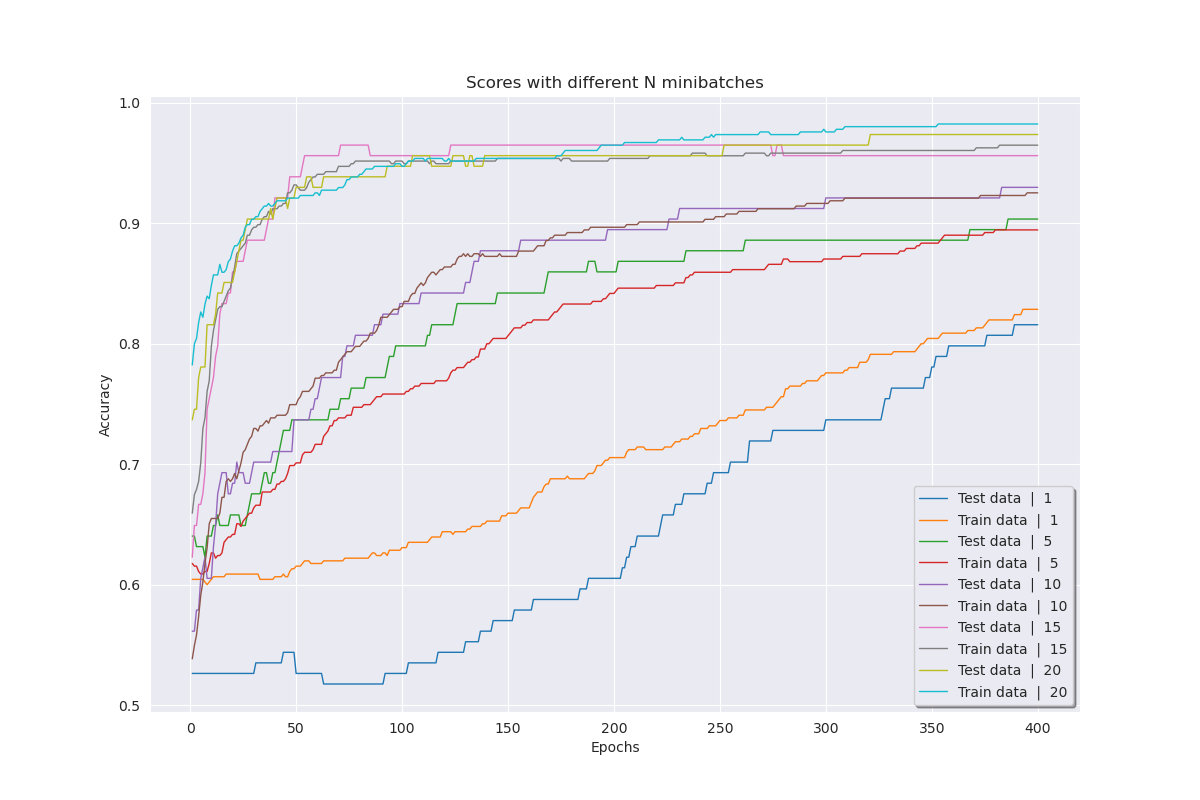
\includegraphics[width=0.8\textwidth]{Figures/PartD/d_line_batch_size.png}
    \caption{Accuracy score for train and test data plottet with respect to epochs for Run 1 (see table
    \ref{tab:runs_classification_cancer}). The number on the labels correspond
to number of mini-batches.}  
    \label{fig:d_line_batch_size} 
\end{figure}


%%%%%%%%%%%%%%% Run 2 %%%%%%%%%%%%%%%
% Lambda vs eta


In figure \ref{fig:d_heatmap_train_eta_vs_lambda} and
\ref{fig:d_heatmap_test_eta_vs_lambda} is accuracy score for run 2 plotted for
different values of regularization parameter and learning rate for the training
and test data respectively. For our test data the best Accuracy of 0.9825 was
gotten with $\lambda = 10^{-4}$, $\eta = 0.1$ and $\lambda = 0.01$, $\eta =
0.01$. Generally we observe that the accuracy tend to increase with increasing
learning rate. This make sense since the model is learning faster. High
learning rates often leads exploding loss scores. This is not observed in this
case. By choosing the largest learning rate, we can maximize the accuracy and
minimize CPU cycles. 

We observe an increasing trend in accuracy with respect to increasing $\lambda $
values (Lambda in figure). This is more significant for the smaller values
of learning rate. To further study this trend we plotted the accuracy score
for different $\lambda $ values with respect to epochs in figure
\ref{fig:_d_line_different_lambdas}. We clearly see in increased convergence
rate for higher values of lambda. Moreover, the accuracy both for the train and
test data is higher for larger values of $\lambda $. For further fine-tuning of
parameters we will set $\lambda = 0$, to better observe how the different
parameters affect the score with respect to epochs. 


% FIXME: fix figures, 

\begin{figure}[H]
    \centering
    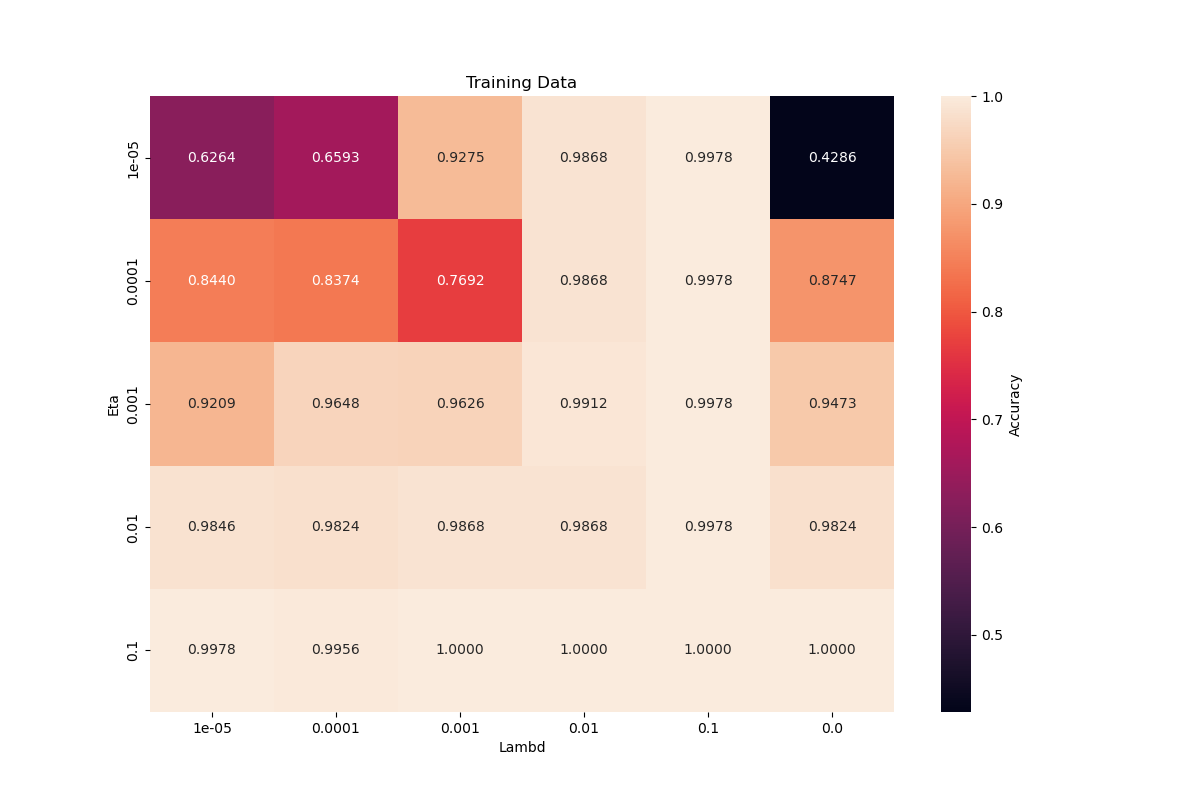
\includegraphics[width=\textwidth]{Figures/PartD/d_heatmap_train_eta_vs_lambda}
    \caption{Heatmap of accuracy score for training dta after 200 epochs with
    respect to different learning rates (Eta) and different L2-regularzation
    parameters (Lambd).   Spesific parameters used in run 2 is listed in table
\ref{tab:runs_classification_cancer}   }  
    \label{fig:d_heatmap_train_eta_vs_lambda}  
\end{figure}

\begin{figure}[H]
    \centering
    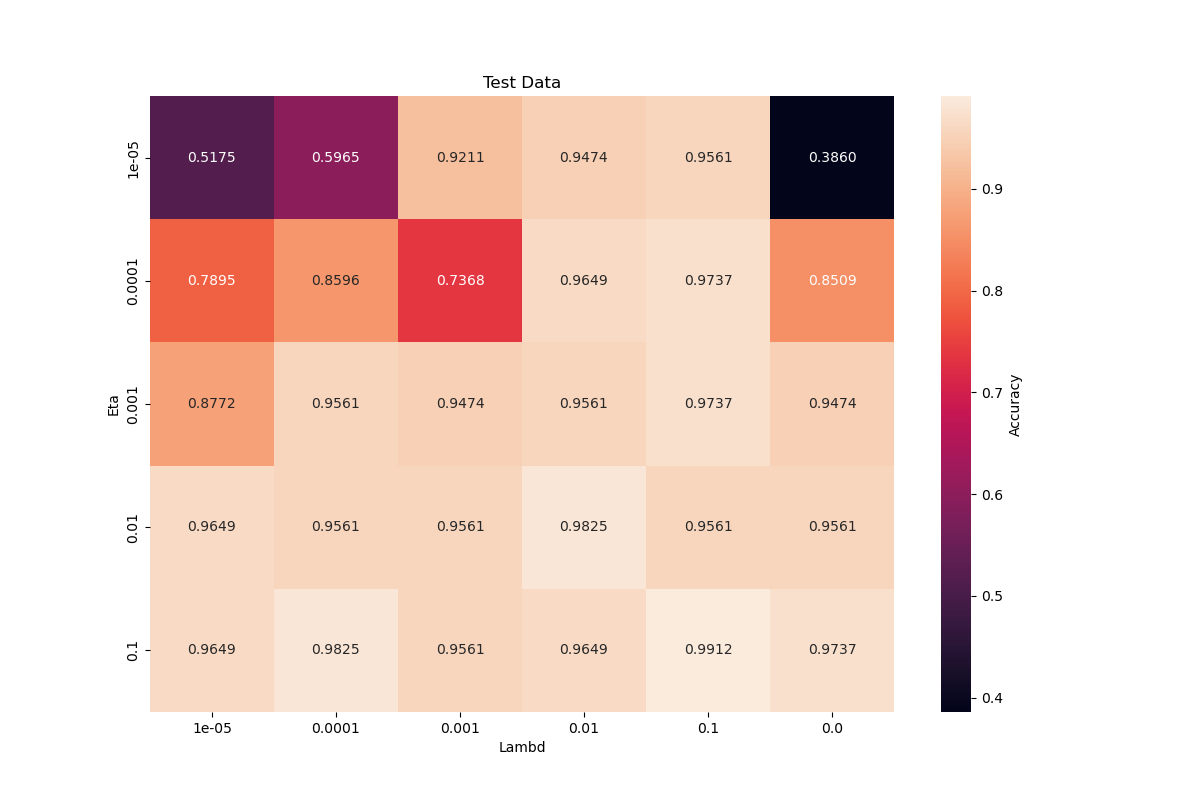
\includegraphics[width=\textwidth]{Figures/PartD/d_heatmap_test_eta_vs_lambda}
    \caption{Heatmap of accuracy score for test dta after 200 epochs with
    respect to different learning rates (Eta) and differn L2-regularization
    parameters (Lambd). Specific parameters used in run 2 is listed in table
    \ref{tab:runs_classification_cancer}       }  
    \label{fig:d_heatmap_test_eta_vs_lambda}  
\end{figure}


            
\begin{figure}[H]
    \centering
    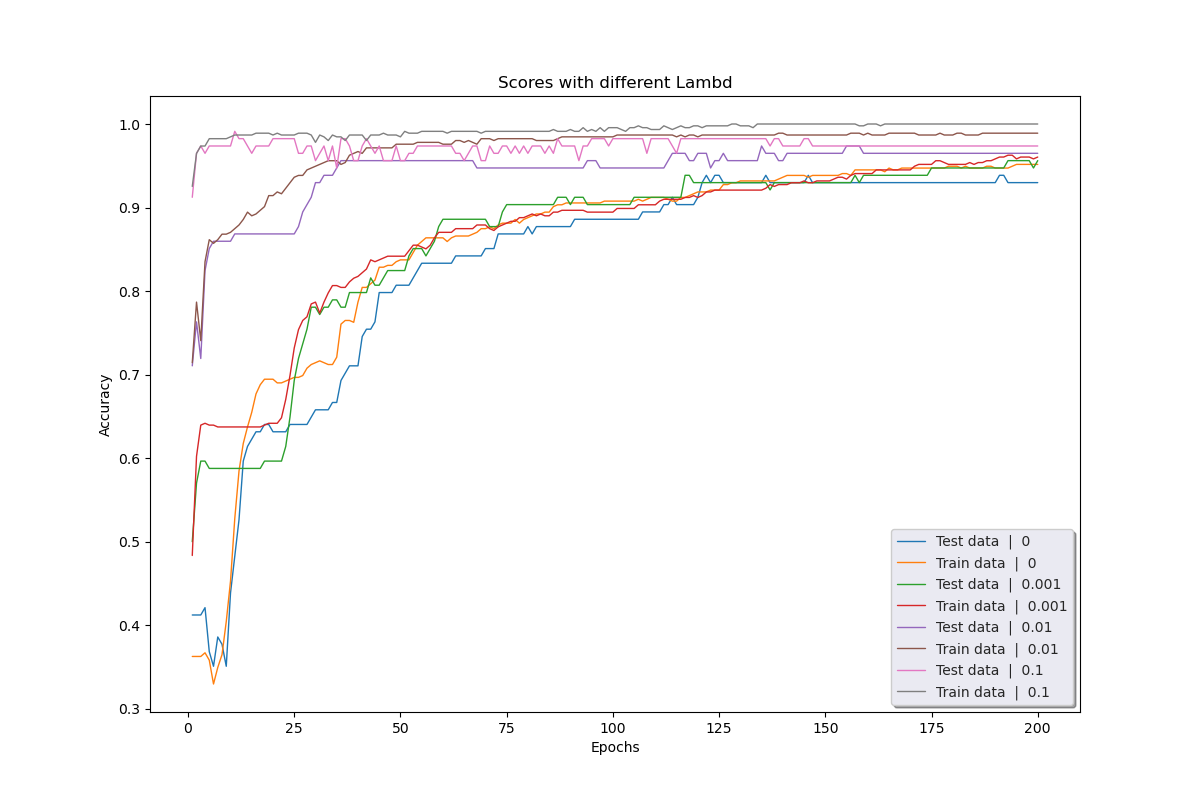
\includegraphics[width=0.8\textwidth]{Figures/PartD/_d_line_different_lambdas.png}
    \caption{Plot of accuracy score for training and test data with respect to
    epochs. Each line correspond to different values of $\lambda $ as indicated
by the number in the legend. A learning rate of 0.001 was used.}  
\label{fig:_d_line_different_lambdas} 
\end{figure}


%%%%%%%%%%%%%%% Run 3 %%%%%%%%%%%%%%%
% Depth vs width


In Run 3 different network architecture was tested with respect number of nodes
(width) and number of hidden layers (depth). The heat map's for the train and test
data is shown in figure \ref{fig:d_heatmap_train_depth_vs_width_lambd_0} and
\ref{fig:_d_heatmap_test_depth_vs_width_lambd_0}. For our test data the best
accuracy score was gotten with 2 hidden layers with 5 nodes in each, with an
accuracy of 0.9912. There is no clear trend with respect to architecture. We
will chose 2 hidden layers and 5 hidden nodes as our best parameters. However
the variations with respect to depth and width, may bet attributed to other random
phenomena such as mini-batch selection. There is no reason to chose a more
complex model since this will increase the computational cost of the network.      

% FIXME: not discussed training data


\begin{figure}[H]
    \centering
    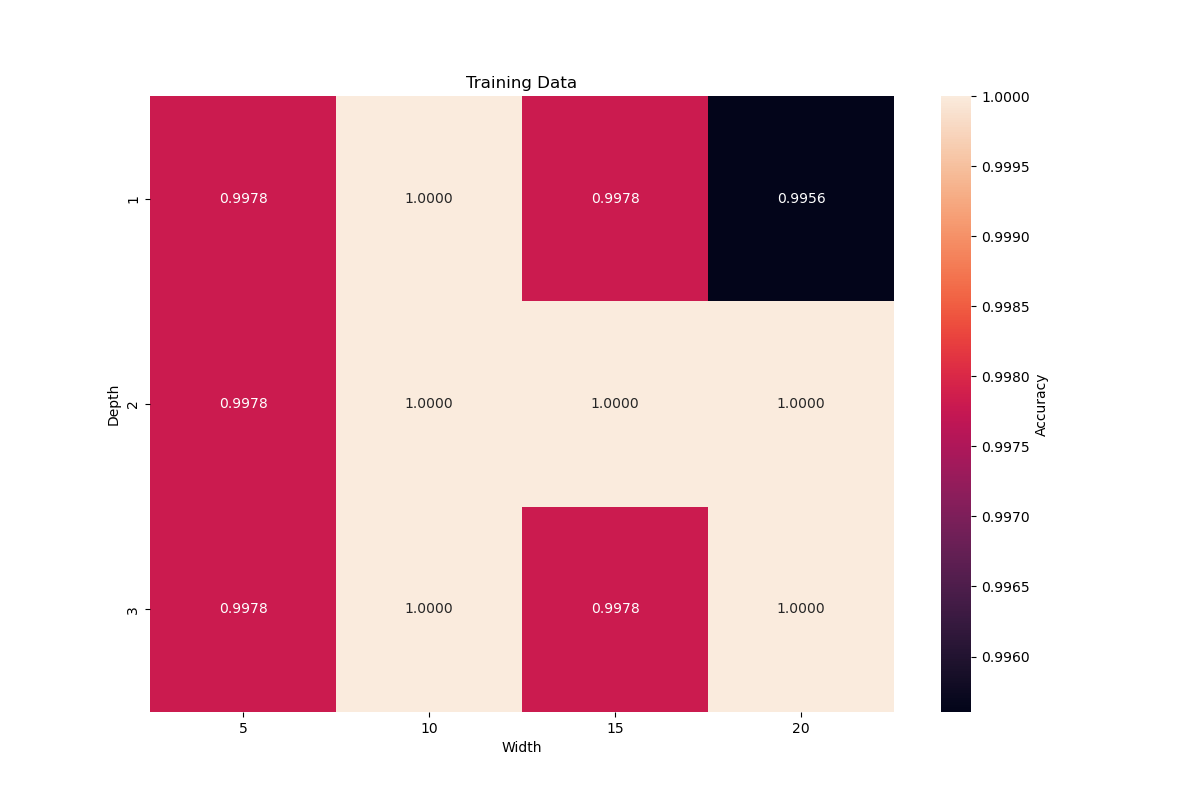
\includegraphics[width=0.8\textwidth]{Figures/PartD/d_heatmap_train_depth_vs_width_lambd_0.png}
    \caption{Accuracy score for train data with respect to different N number
        of hidden layers (depth) and number of hidden nodes in each hidden layer
    (width)  }  
    \label{fig:d_heatmap_train_depth_vs_width_lambd_0} 
\end{figure}


\begin{figure}[H]
    \centering
    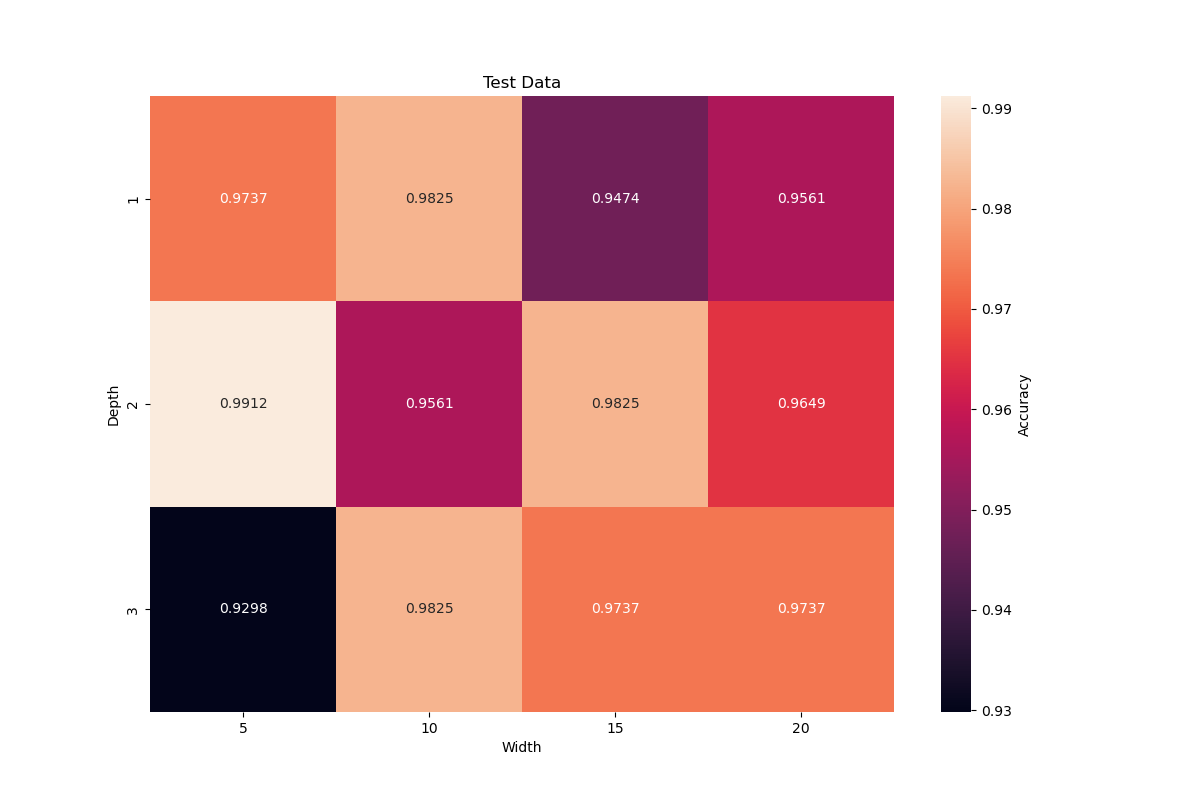
\includegraphics[width=0.8\textwidth]{Figures/PartD/_d_heatmap_test_depth_vs_width_lambd_0.png}
    \caption{Accuracy score for test data with respect to different N number
        of hidden layers (depth) and number of hidden nodes in each hidden layer
    (width)  }  
    \label{fig:_d_heatmap_test_depth_vs_width_lambd_0} 
\end{figure}

%%%%%%%%%%%%%%% Run 4 %%%%%%%%%%%%%%%
% Testing tuning method width and without momentum  

In Run 4 we tested different learning rate tuning methods. In figure
\ref{fig:d_tuning_eta_0_001_with_gamma_0} the accuracy score is plotted
with respect to epochs for manual (none), adagrad, adman and the rms prop
tuning method. The learning rate parameter was set to 0.001. We observe that
RMS Prop and ADAM converges much faster than Adagrad and without any tuning.
The poor performance of Adgrad is probably due the low value initial value for
$\eta $. Both ADAM and RMS-prop performance well on both the training and test
data with a high accuracy and convergence after around 50 epochs. 

In figure \ref{fig:d_tuning_eta_0_001_with_gamma_0_9} the same lines are
plotted but with momentum, $\gamma = 0.9$. This causes a significant
improvement both the accuracy and convergence rate with Adagrad and plain SGD.   
Adagrad gives better prediction on the test data than both RMS prop and ADAM.
The added momentum to ADAM causes more fluctuations with respect to epochs than
without momentum.  

\begin{figure}[H]
    \centering
    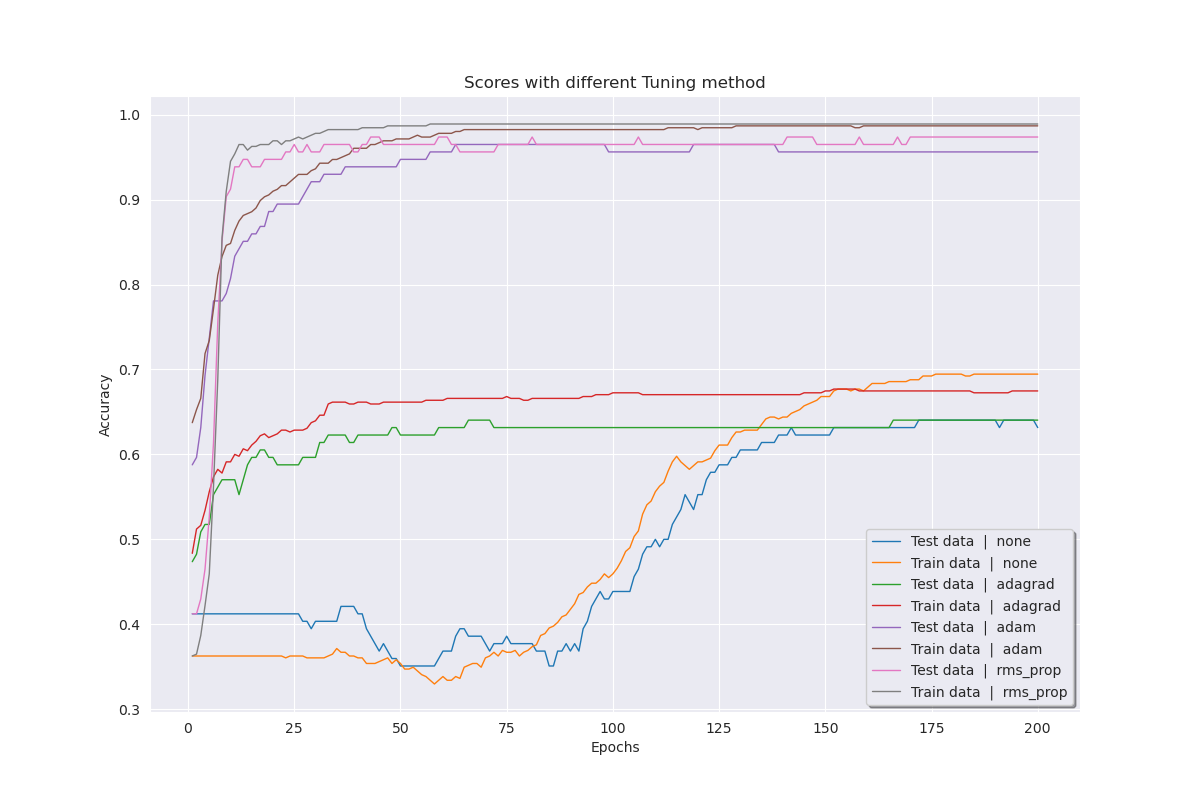
\includegraphics[width=0.8\textwidth]{Figures/PartD/d_tuning_eta_0_001_with_gamma_0.png}
    \caption{Accuracy score for test and data with different tuning methods
    plotted as function of epochs. Momentum ($\gamma $) is set to 0.}  
    \label{fig:d_tuning_eta_0_001_with_gamma_0} 
\end{figure}


\begin{figure}[H]
    \centering
    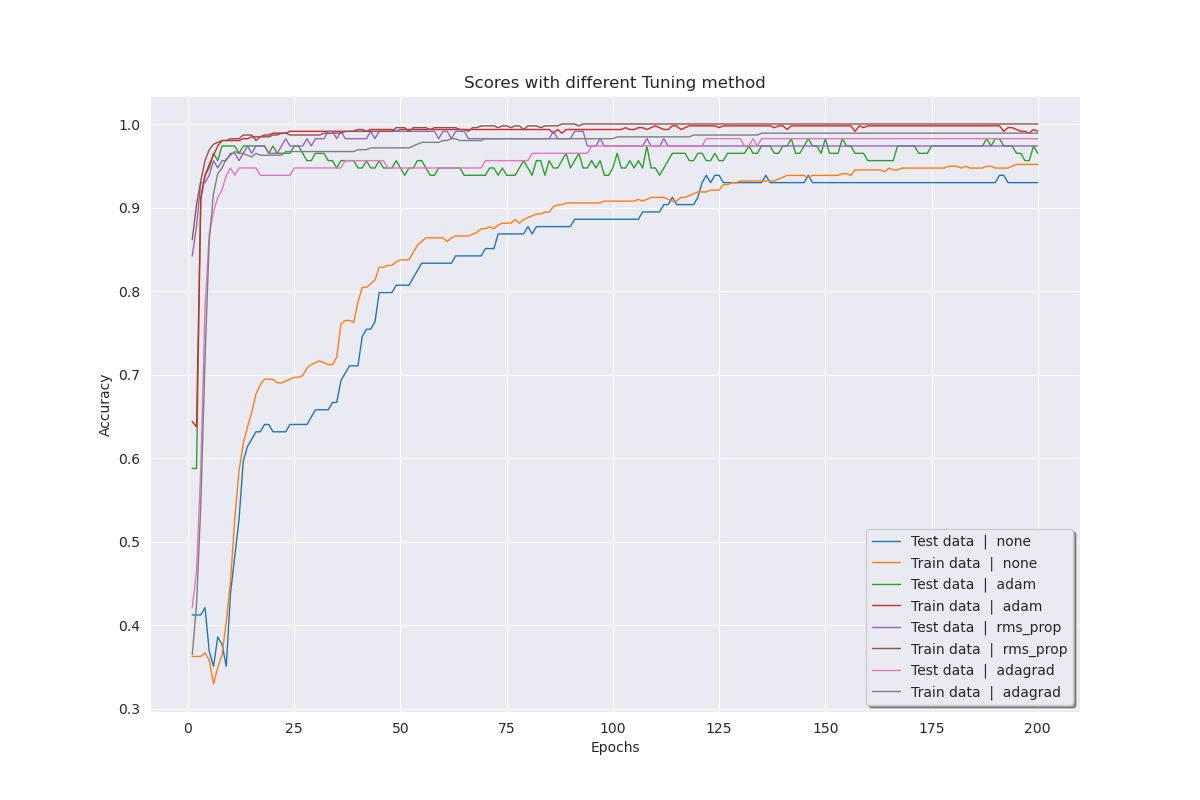
\includegraphics[width=0.8\textwidth]{Figures/PartD/d_tuning_eta_0_001_with_gamma_0_9.png}
    \caption{Accuracy score for test and data with different tuning methods
    plotted as function of epochs. Momentum ($\gamma $) is set to 0.9.}  
    \label{fig:d_tuning_eta_0_001_with_gamma_0_9} 

\end{figure}

%%%%%%%%%%%%%%% Run 5 %%%%%%%%%%%%%%%
% Activation function on hidden layers 

In run 5 we tested different activation functions on the hidden. From run 4 we
observed that both tuning method and added momentum improved the results
significantly. To understand better the different activation functions affect
the results we used a momentum parameter $\gamma = 0$ with constant learning
rate, $\eta = 0.001$. In figure \ref{fig:d_line_activation_hidden_gamma_0} the
accuracy is plotted for different activation functions in the hidden layers.
Both RELU and leaky RELU outperforms the sigmoid activation function. RELU and
Leaky RELU performs similar on the training data, but RELU gives the best
overall accuracy on the test data. 


\begin{figure}[H]
    \centering
    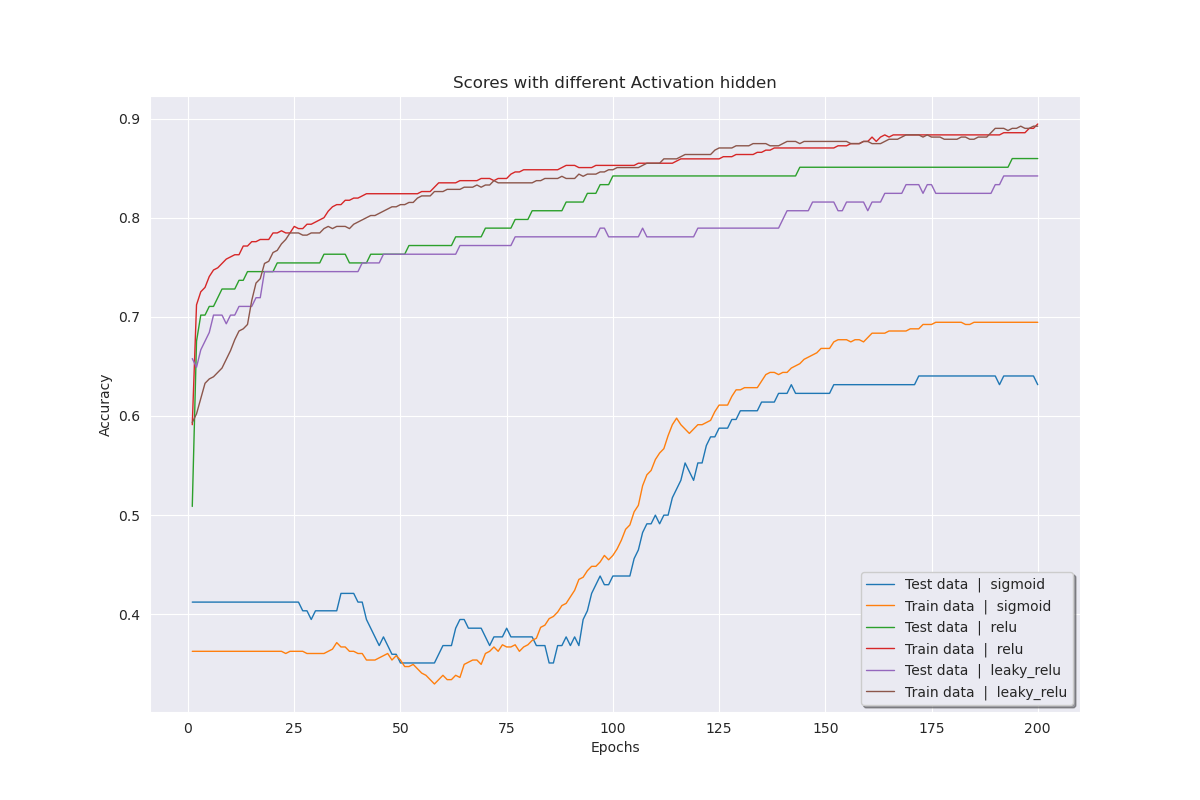
\includegraphics[width=0.8\textwidth]{Figures/PartD/d_line_activation_hidden_gamma_0.png}
    \caption{Accuracy score for train and test data with respect to epochs.
    Different activation functions on the hidden layers was used as indicated
in the label}  
\label{fig:d_line_activation_hidden_gamma_0} 
\end{figure}


%%%%%%%%%%%%%%% Run 6 %%%%%%%%%%%%%%%
% Combine best parameters

In run 6 our model reached an accuracy of 0.9825 after 165 epochs (see figure
\ref{fig:d_line_best}). The result was stable
with increasing number of iterations. We tried to select the optimal values for
hyper-parameters on the basis of the previous experimentation. However, we did
use the sigmoid function on the hidden layers and not REL or Leaky REL, as
they performed worse. The parameters used in run 6 is listed in table
\ref{tab:runs_classification_cancer2}. 

The overall best accuracy score on the test data seen in this experiment was observed in Run
3, where we experimented with different network architecture. Then we got a
score of 0.9912. We suspected that this was due to luck and random events in
our mini-batch selection method. 
% Compare with keras
Overall our model seemed to perform really well on a Classification problem
with the Wisconsin Breast Cancer data. We compared our results from run 6 with Kares
(python API for Tensor Flow), With the exact same parameters, except $\eta =
1$ and $\gamma = 0$. We then got a test accuracy prediction of 0.9825, that
matches our finding. 


% improvements
We originally tried to find the optimal parameters of the Network, by improving
a few parameters at the time. However, our best parameter choices created a
model with excellent predations after only a few epochs. Therefore, we decided
to remove some of the parameters to better be able to study how each individual
parameter affected the model. However, there is not certain that all the
parameters will play nicely together. Thus, a more methodical approach should
have been applied in order to see how different parameters affect each other.     


From the literature we found
that models created with an artificial neural network and random forest
produces test accuracy's of 92.44 and 95.64 respectively \cite{Vig2014ComparativeAO}. Our model does a
better job on the test data. We don't expect our simple FINN code to be
superior to others. However, we do not suspect any error in implementation
since our benchmarking gave the same result.   

There is one serious drawback with our approach. We did not use any re-sampling
technique when we trained our model. Our high accuracy score is probably due to
our specific train-data subset selection. Bootstrap re-sampling would have been
a good choice to better control the randomness in our model. Then we would have
got better insight model variation due to parameter selection, and not random
events. However, this approach would have been too expensive for our
laptops. Therefore, a re-sampling technique such as k-fold cross validation
should have been applied.  

To better control the randomness in our model we should have predefined a
mini batch sequence, and also used the same initial weights when this was
possible. Then we could have more easily seen if the variations in our
predictions was due to random events or not. We did not study how the weights
and bias initialization affected the results. Insight in how random events
affected our model could have been obtained by applying Bootstrap re-sampling. 

\begin{figure}[H]
    \centering
    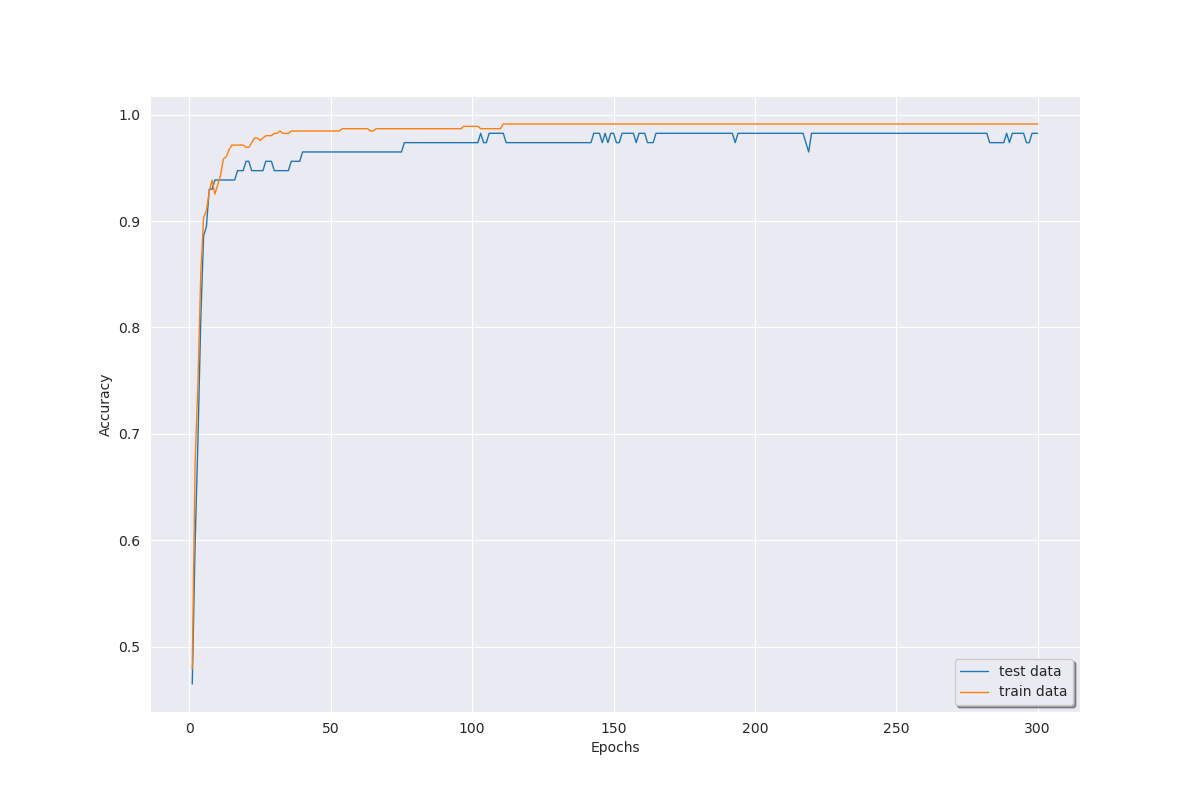
\includegraphics[width=0.8\textwidth]{Figures/PartD/d_line_best.png}
    \caption{Run 6: Plot of accuracy score for train and test data, where we
    tried to find the overall best hyperparameter combination}  
    \label{fig:d_line_best} 
\end{figure}


After all these calculations there is only a few obvious choices for
hyperparameters. A larger number of mini-batches did increase the accuracy,
convergence rate and reduces required CPU cycles. We did not observe any over-fitting in 
our model, but a larger value of lambda did increase the convergence rate.
There was no clear trend in accuracy score with respect to network
architecture, but a depth of 2 and width of 5 gave the best prediction on the
test data. Tuning methods such as Adam and RMS prop, significantly improved the
convergence rate. Adagrad and manual tuning was inferior to rms prop and adam,
but significantly improved when momentum was added. Adagrad then performed the
best on the test data. 


%  ____            _          
% |  _ \ __ _ _ __| |_    ___ 
% | |_) / _` | '__| __|  / _ \
% |  __/ (_| | |  | |_  |  __/
% |_|   \__,_|_|   \__|  \___|
                            

%%%%%%%%%%%%%%%%%%%%%%%%%%%%%%%%%%%%%%%%%%%%%
\subsection{Logistic regression}
% Study the results as functions of teh chosen learning rates 
% Add l2 regularization

In figure the accuracy score obtained with logistic regression is plotted for
different number of mini-batches. Again a small mini-batch size seems to be the
obvious choice as discussed for our neural network. In figure
\ref{fig:e_heatmap_train_lambd_vs_eta_gamma_0_9_epochs_200} and
\ref{fig:e_heatmap_test_lambd_vs_eta_gamma_0_9_epochs_200} the accuracy on the
Cancer Data is plotted with different learning rates and L2-regularization
parameters for the train and test data respectively. The best score for both
the training and test data was obtained with a learning rate $\eta = 0.001$
without any regularization. Our best prediction on the test data got an
accuracy of 0.9035. Our neural network code does contain 11 times as many
weights. Thus, we expect it to be able to produce more complex patterns. 
With did benchmark our result against scikit-learn's Logistic regression
method. We then got a test accuracy of  0.9649. We was not able to improve our
logistic regression algorithm to produce this result. We do not suspect that
our implementation is wrong. Scikit-learn's may contain further optimization.
Hence, the better accuracy score. However, our Neural Network did produce a
better accuracy score than Scikit-learns logistic regression method.

\begin{figure}[H]
    \centering
    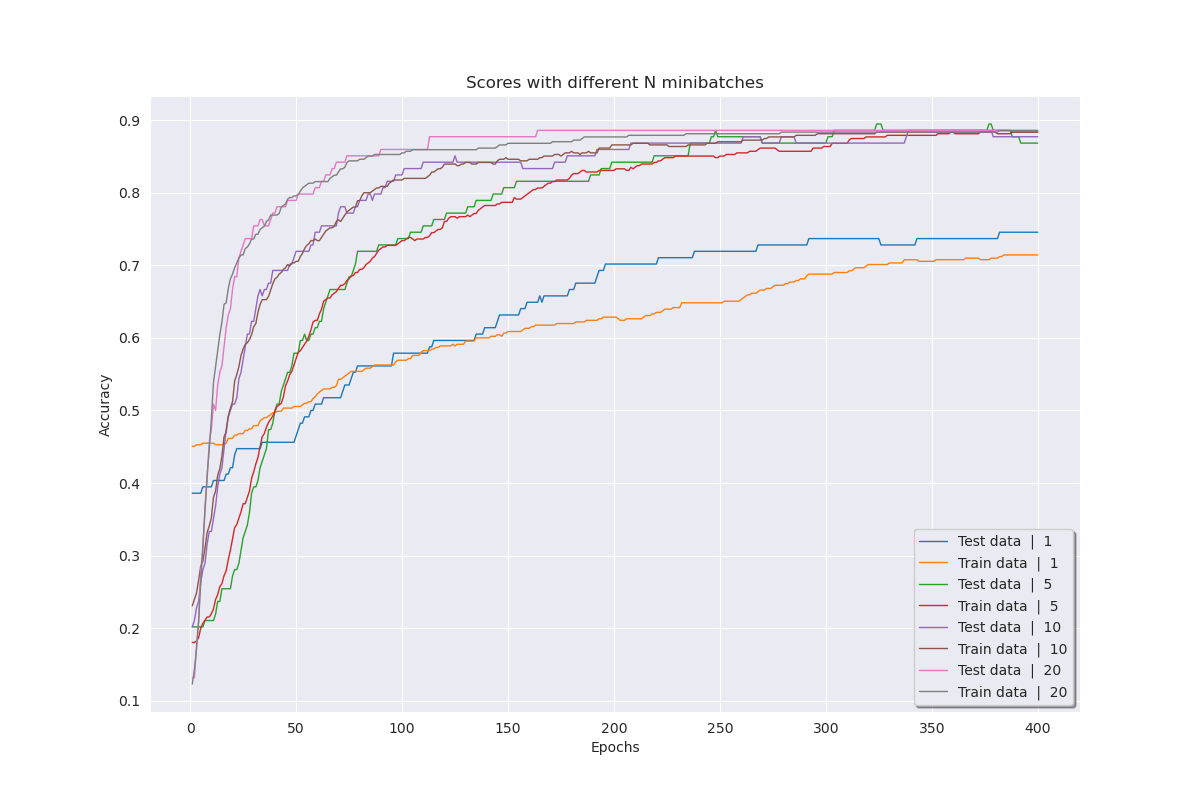
\includegraphics[width=0.8\textwidth]{Figures/PartE/e_line_n_minibatches_gamma_0_9.png}
    \caption{fig:Accuracy score obtained with logistic regression on the
        Wisconsin Breast Cacner data. Predication on training and test data is
    plotted for different number of mini-batches as indicated in the label.}  
    \label{fig:e_line_n_minibatches_gamma_0_9} 

\end{figure}

\begin{figure}[H]
    \centering
    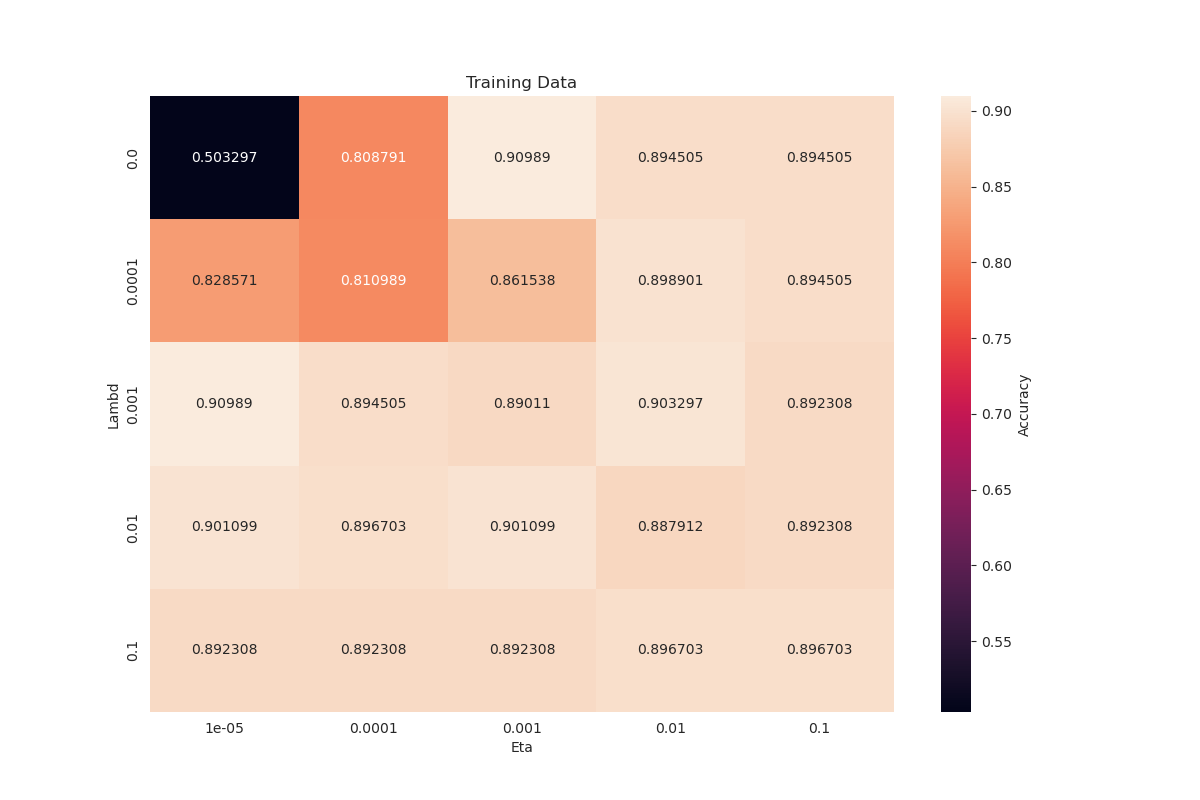
\includegraphics[width=0.8\textwidth]{Figures/PartE/e_heatmap_train_lambd_vs_eta_gamma_0_9_epochs_200.png}
    \caption{Accuracy score on Wisconsin Breast Cancer training data, with
    respect to different learning rates and L2 regularization parameters.}  
    \label{fig:e_heatmap_train_lambd_vs_eta_gamma_0_9_epochs_200} 
\end{figure}


\begin{figure}[H]
    \centering
    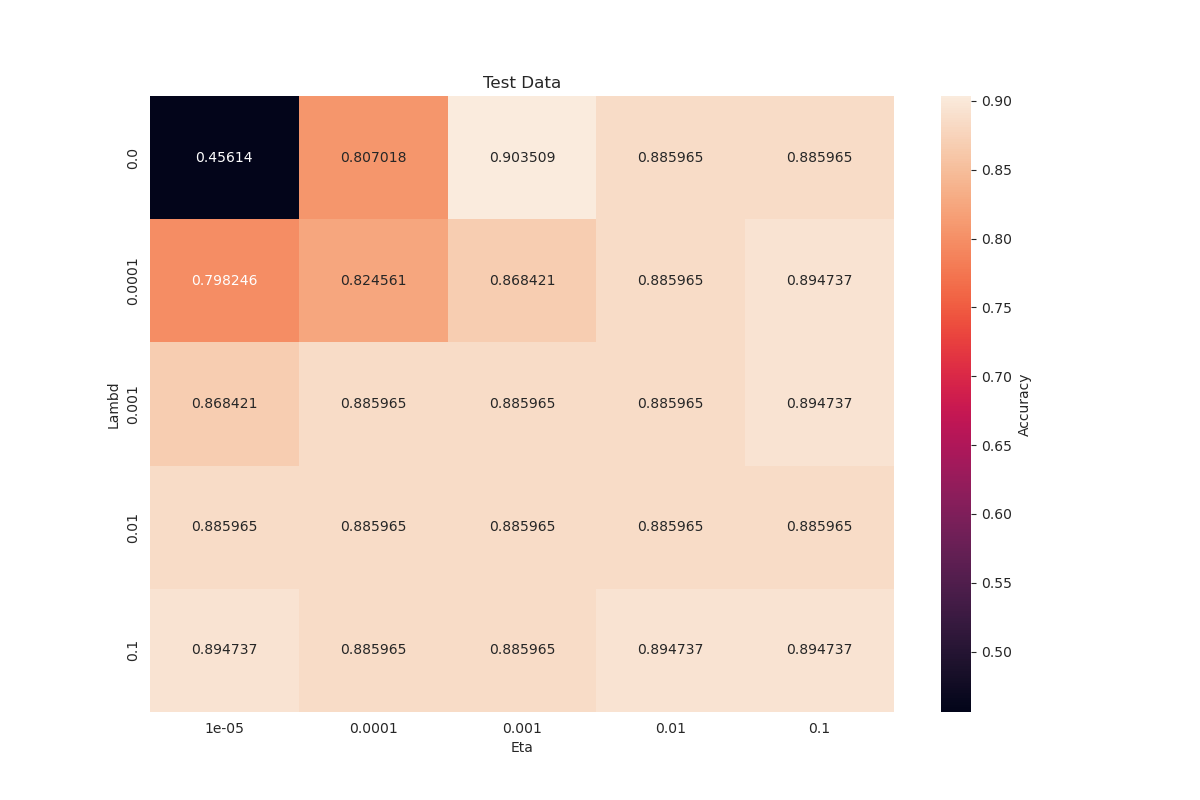
\includegraphics[width=0.8\textwidth]{Figures/PartE/e_heatmap_test_lambd_vs_eta_gamma_0_9_epochs_200.png}
    \caption{Accuracy score on Wisconsin Breast Cancer test data, with
    respect to different learning rates and L2 regularization parameters.}  
    \label{fig:e_heatmap_test_lambd_vs_eta_gamma_0_9_epochs_200} 
\end{figure}


%%%%%%%%%%%%%%%%%%%%%%%%%%%%%%%%%%%%%%%%%%%%%
\subsection{Error in L2-regularzation} \label{sec:error_l2_regularization} 
After our report was completed and ready for delivery we found an error in how
the L2 regularization parameter was calculated. Instead of multiplying the
regularization parameter with our weights from our previous iteration, the
regularization parameters was multiplied with the gradient of the weights,
effectively increasing the learning rate. Our analysis of the L2 regularization
parameter is therefore not valid.









